% ===============================================================
%  ME249 Fall 2026 -- Project 2 -- Summary report
%  Compile with:  pdflatex report.tex  (twice, for the table of contents and references)
% ===============================================================
\documentclass[11pt]{article}

\newcommand{\studentname}{Adnan AHALI}

% ---------------------------------------------------------------
%  Preamble - ME249 Project 2 report
% ---------------------------------------------------------------
\usepackage[T1]{fontenc}
\usepackage[utf8]{inputenc}
\usepackage{lmodern}
\usepackage[a4paper,margin=2.3cm]{geometry}
\usepackage{amsmath,amssymb}
\usepackage{graphicx}
\usepackage{booktabs}
\usepackage{multirow}
\usepackage{array}
\usepackage{tabularx}
\usepackage{adjustbox}
\usepackage{float}
\usepackage{caption}
\usepackage{subcaption}
\usepackage[dvipsnames,table]{xcolor}
\usepackage{enumitem}
\usepackage{listings}
\usepackage{fancyhdr}
\usepackage{textcomp}
\usepackage[hidelinks,hypertexnames=false]{hyperref}

\captionsetup{font=small, labelfont=bf, margin=0.5cm}
\setlist{itemsep=1pt, topsep=3pt}
\setlength{\parskip}{3pt}
\setlength{\emergencystretch}{3em}
\renewcommand{\arraystretch}{1.15}

\definecolor{codebg}{HTML}{F7F7F5}
\definecolor{codecomment}{HTML}{52514E}
\definecolor{codekw}{HTML}{1C5CAB}
\definecolor{codestr}{HTML}{A33A1A}
\definecolor{good}{HTML}{006300}
\definecolor{bad}{HTML}{B02A2A}

\lstdefinestyle{py}{
  language=Python,
  basicstyle=\ttfamily\scriptsize,
  keywordstyle=\color{codekw}\bfseries,
  commentstyle=\color{codecomment}\itshape,
  stringstyle=\color{codestr},
  backgroundcolor=\color{codebg},
  numbers=left, numberstyle=\tiny\color{codecomment}, numbersep=6pt,
  frame=single, rulecolor=\color{black!15},
  breaklines=true, breakatwhitespace=false, columns=fullflexible, keepspaces=true,
  showstringspaces=false, tabsize=4,
  literate={°}{{\textdegree}}1 {±}{{$\pm$}}1 {–}{{--}}1
}
\lstset{style=py}

\pagestyle{fancy}
\fancyhf{}
\lhead{\small ME249 Fall 2026 -- Project 2}
\rhead{\small \studentname}
\cfoot{\small \thepage}
\renewcommand{\headrulewidth}{0.4pt}
\setlength{\headheight}{14pt}

% notation
\newcommand{\qpp}{q''}
\newcommand{\dTsat}{(T_w-T_{sat})}
\newcommand{\Ferrmean}{[F_{err}]_{mean}}
\newcommand{\gen}{g_{en}}
\newcommand{\code}[1]{\texttt{#1}}
\newcommand{\nh}[1]{\hat{n}_{#1}}
\newcommand{\fittable}[1]{\begin{adjustbox}{max width=\linewidth}\input{tables/#1}\end{adjustbox}}

% generated from code/results/*.json
\newcommand{\TwoOneMlow}{2.94}
\newcommand{\TwoOneClow}{1.73\times10^{-3}}
\newcommand{\TwoOneMhigh}{2.80}
\newcommand{\TwoOneChigh}{2.95\times10^{-3}}
\newcommand{\TwoTwoNone}{1.72\times10^{-3}}
\newcommand{\TwoTwoNtwo}{2.9747}
\newcommand{\TwoTwoNthree}{0.0438}
\newcommand{\TwoTwoF}{0.02870}
\newcommand{\TwoTwoRefF}{0.02869}
\newcommand{\TwoTwoRefNone}{1.51\times10^{-3}}
\newcommand{\TwoTwoRefNtwo}{3.0103}
\newcommand{\TwoTwoRefNthree}{0.0464}
\newcommand{\TwoTwoBaseF}{0.03084}
\newcommand{\TwoTwoBaseKconv}{12}
\newcommand{\TwoTwoBaseKmin}{5202}
\newcommand{\TwoTwoRmsAbs}{23.1}
\newcommand{\TwoTwoRmsRel}{16.6}
\newcommand{\TwoTwoMeanAbsRel}{13.2}
\newcommand{\TwoTwoMaxRel}{33}
\newcommand{\TwoTwoWithin}{47}
\newcommand{\TwoTwoMeanQ}{113}
\newcommand{\TwoTwoBiasLow}{-1.8}
\newcommand{\TwoTwoRmsLow}{7.5}
\newcommand{\TwoTwoBiasMid}{-19.2}
\newcommand{\TwoTwoRmsMid}{20.2}
\newcommand{\TwoTwoBiasHigh}{+15.7}
\newcommand{\TwoTwoRmsHigh}{20.8}
\newcommand{\TwoTwoBestSet}{Set 2}
\newcommand{\TwoTwoBestSeed}{2}
\newcommand{\TwoThreeNone}{1.20\times10^{-4}}
\newcommand{\TwoThreeRefNone}{1.56\times10^{-4}}
\newcommand{\TwoThreeNtwo}{3.0216}
\newcommand{\TwoThreeRefNtwo}{2.9771}
\newcommand{\TwoThreeNthree}{0.4619}
\newcommand{\TwoThreeRefNthree}{0.4808}
\newcommand{\TwoThreeNfour}{1.3485}
\newcommand{\TwoThreeRefNfour}{1.2586}
\newcommand{\TwoThreeNfive}{0.5435}
\newcommand{\TwoThreeRefNfive}{0.4708}
\newcommand{\TwoThreeF}{0.02097}
\newcommand{\TwoThreeFval}{0.02566}
\newcommand{\TwoThreeRefF}{0.02085}
\newcommand{\TwoThreeFinit}{0.03212}
\newcommand{\TwoThreeBaseF}{0.02808}
\newcommand{\TwoThreeBaseKmin}{2309}
\newcommand{\TwoThreeBaseKconv}{193}
\newcommand{\TwoThreeRmsTrain}{12.3}
\newcommand{\TwoThreeRmsVal}{14.1}
\newcommand{\TwoThreeMadTrain}{9.4}
\newcommand{\TwoThreeMadVal}{10.9}
\newcommand{\TwoThreeWithinTrain}{58}
\newcommand{\TwoThreeWithinVal}{53}
\newcommand{\TwoThreeRmsAbsTrain}{17.2}
\newcommand{\TwoThreeRmsAbsVal}{15.0}
\newcommand{\TwoThreeBestSet}{C}
\newcommand{\TwoThreeBestSeed}{1}
\newcommand{\TwoThreeGeq}{23.7}
\newcommand{\TwoThreeGeqRatio}{2.4}
\newcommand{\TwoThreeBiasOneG}{-16}
\newcommand{\TwoThreeBiasTwoG}{+11}
\newcommand{\TwoThreeBiasOthersMin}{-4}
\newcommand{\TwoThreeBiasOthersMax}{+6}
\newcommand{\EtOneSdT}{3.18}
\newcommand{\EtOneSg}{0.135}
\newcommand{\EtOneSgam}{0.324}
\newcommand{\EtOneSP}{0.537}
\newcommand{\EtOneWorst}{3.6}
\newcommand{\EtOneRss}{4.6}
\newcommand{\EtOneSingle}{4.7}
\newcommand{\EtOneWorstC}{1.4}
\newcommand{\EtOneSingleC}{1.9}
\newcommand{\EtOneCheck}{15.3}
\newcommand{\EtOneSgLow}{0.0019}
\newcommand{\EtOneSgamLow}{0.454}
\newcommand{\EtTwoSigma}{0.126}
\newcommand{\EtTwoGaF}{0.00843}
\newcommand{\EtTwoImpF}{0.00865}
\newcommand{\EtTwoNoiseFreeF}{2.7\times10^{-6}}
\newcommand{\EtTwoDiffOne}{+2.1}
\newcommand{\EtTwoDiffRefOne}{+6.9}
\newcommand{\EtTwoDiffTwo}{-7.1}
\newcommand{\EtTwoDiffRefTwo}{-8.4}
\newcommand{\EtTwoDiffThree}{+4.8}
\newcommand{\EtTwoDiffRefThree}{+10.5}
\newcommand{\EtTwoDiffFour}{-3.0}
\newcommand{\EtTwoDiffRefFour}{+5.7}
\newcommand{\EtTwoDiffFive}{+17.4}
\newcommand{\EtTwoDiffRefFive}{+4.3}
\newcommand{\TwoFiveNone}{5.705}
\newcommand{\TwoFiveNtwo}{5.425}
\newcommand{\TwoFiveNthree}{1.130}
\newcommand{\TwoFiveFtrain}{0.0166}
\newcommand{\TwoFiveFval}{0.0208}
\newcommand{\TwoFiveFall}{0.0174}
\newcommand{\TwoFiveUA}{2.907}
\newcommand{\TwoFiveHr}{6.55}
\newcommand{\TwoFiveKmin}{9160}
\newcommand{\TwoFiveBestSet}{Set 3}
\newcommand{\TwoFiveBestNgen}{20000}
\newcommand{\TwoFiveBestSeed}{1}
\newcommand{\TwoFiveRefF}{0.01659}
\newcommand{\TwoFiveRefFval}{0.0208}
\newcommand{\TwoFiveRefNone}{26.40}
\newcommand{\TwoFiveRefNtwo}{3.114}
\newcommand{\TwoFiveRefNthree}{0.598}
\newcommand{\TwoFiveNconv}{54}
\newcommand{\TwoFiveConvNoneMin}{4.96}
\newcommand{\TwoFiveConvNoneMax}{11.28}
\newcommand{\TwoFiveConvNtwoMin}{3.44}
\newcommand{\TwoFiveConvNtwoMax}{6.11}
\newcommand{\TwoFiveConvNthreeMin}{0.67}
\newcommand{\TwoFiveConvNthreeMax}{2.84}
\newcommand{\TwoFiveConvUAMin}{2.893}
\newcommand{\TwoFiveConvUAMax}{2.911}
\newcommand{\TwoFiveProfMaxF}{0.016591}
\newcommand{\TwoFiveProfMinF}{0.016588}


\begin{document}

% ---------------------------------------------------------------- title page
\begin{titlepage}
\centering
\vspace*{1.5cm}
{\large University of California, Berkeley -- Mechanical Engineering Department\par}
\vspace{0.4cm}
{\large ME249, Fall 2026 -- Prof.\ V.~P.~Carey\par}
\vspace{2.2cm}
\rule{\linewidth}{0.6pt}\\[0.5cm]
{\LARGE\bfseries Project 2\par}
\vspace{0.4cm}
{\Large Genetic-algorithm modelling of nucleate boiling of a water/2-propanol mixture in variable gravity,
and calibration of a heat-pipe heat-exchanger model\par}
\vspace{0.3cm}
\rule{\linewidth}{0.6pt}\\[1.6cm]
{\large \studentname\par}
\vspace{0.4cm}
{\large Individual project (team of one)\par}
\vfill
{\large Report due October 27, 2026\par}
\end{titlepage}

% ---------------------------------------------------------------- summary
\section*{Summary}
\addcontentsline{toc}{section}{Summary}
All tasks of Project~2 were completed, including those that individuals working alone may omit
(Task~2.1(b), Task~2.3) and the extra tasks ET1 and ET2 assigned to teams of three. The genetic algorithm
(GA) of the skeleton programs was kept, but one bug of the skeleton code and two data values had to be
corrected. The main results are:

\begin{table}[H]
\centering\small
\begin{tabularx}{\linewidth}{@{}l X c@{}}
\toprule
Task & Best-fit relation (GA) & Error (target)\\
\midrule
2.2 & $\qpp=\TwoTwoNone\,\dTsat^{\TwoTwoNtwo}\,g^{\TwoTwoNthree}$ & $\Ferrmean=\TwoTwoF$ ($<0.035$)\\
2.3 & $\qpp=\TwoThreeNone\,\dTsat^{\TwoThreeNtwo}(g+\TwoThreeNfour\,\gen\gamma)^{\TwoThreeNthree}P^{\TwoThreeNfive}$ & $\TwoThreeF$ ($<0.03$); validation $\TwoThreeFval$\\
ET2 & $\dTsat=20.27\,(\qpp)^{0.3074}(g+1.308\,\gen\gamma)^{-0.1455}P^{-0.1485}$ & $\EtTwoGaF$\\
2.5 & $(UA)_e=\TwoFiveNone$~W/\textdegree C, $(UA)_c=\TwoFiveNtwo$~W/\textdegree C, $\alpha=\TwoFiveNthree$ & MAE $\TwoFiveFtrain$ / $\TwoFiveFval$ ($<0.045$)\\
\bottomrule
\end{tabularx}
\end{table}

The three-constant power law of Task~2.2 fits the data only to $\pm\TwoTwoRmsRel\,\%$ (rms), which is
worse than the $\pm10\,\%$ data uncertainty, because it cannot describe the Marangoni effect. The
five-constant model of Task~2.3 brings the overall deviation close to the noise level ($\TwoThreeRmsTrain\,\%$),
although the $1\,\gen$ and $2\,\gen$ (5.5~kPa) groups keep a bias of $11$--$16\,\%$.
It shows that for $\gamma=1.79$ the Marangoni flow acts like an extra gravity of about $2.4\,\gen$. For the
heat pipe, the data determine only the overall conductance $UA_{eff}=\TwoFiveUA$~W/\textdegree C, not $(UA)_e$ and
$(UA)_c$ separately. About 300 GA runs show that the most important property of the initial guesses is
that the output they predict has the right order of magnitude. Far from the solution, the GA either
stagnates (steps that are too small along a narrow valley) or freezes completely (the relative selection
threshold keeps no survivor). Larger mutations, followed by a refinement with small mutations, and a
larger selection fraction solve these problems.

\tableofcontents
\newpage

% ===============================================================
\section{Introduction and organisation of the work}
% ===============================================================

This report documents the work done for Project~2 of ME249. In Part~1, a genetic algorithm (GA) is used to
extract, from nucleate boiling data obtained for a water/2-propanol mixture at gravity levels between
$0.01\,\gen$ and $2\,\gen$, the dependence of the heat flux on wall superheat, gravity, Marangoni
(surface-tension) effects and pressure. In Part~2, the same GA is adapted to calibrate a simple
performance model of a heat-pipe heat exchanger that cools an electronics cabinet.

\subsection{Division of the work}
\label{sec:division}

\textbf{I worked alone on this project}, so all tasks (programming, runs, analysis, figures and report)
were done by me. The adjustment sheet for individuals working alone allows omitting part~(b) of
Task~2.1 and Task~2.3. The two extra tasks ET1 and ET2 are assigned to teams of three. \textbf{I still
completed the whole project}: Tasks~2.1(a) and (b), 2.2, 2.3, ET1, ET2, 2.4, 2.5 and 2.6.

\begin{table}[H]
\centering\small
\caption{Tasks, programs and where the results are reported. All programs are Jupyter notebooks in the
folder \code{code/}. Their full listings are in Appendix~\ref{app:code}.}
\label{tab:tasks}
\begin{tabularx}{\linewidth}{@{}l l X l@{}}
\toprule
Task & Program (notebook) & Content & Section\\
\midrule
2.1 (a), (b) & \code{P2\_Task2.1.ipynb}      & data check, log-log plot of $\qpp$ vs.\ superheat & \ref{sec:t21}\\
2.2          & \code{P2\_Task2.2.ipynb}      & three-constant model, Eq.~(1.1), 45 points & \ref{sec:t22}\\
2.3          & \code{P2\_Task2.3.ipynb}      & five-constant model, Eq.~(1.5), 77 + 15 points & \ref{sec:t23}\\
ET1          & \code{P2\_ET1.ipynb}          & fractional sensitivity of $\qpp$ to its inputs & \ref{sec:et1}\\
ET2          & \code{P2\_ET2.ipynb}          & inverse relation for the superheat, Eq.~(ET2.1) & \ref{sec:et2}\\
2.4, 2.5     & \code{P2\_Task2.4-2.5.ipynb}  & heat-pipe model, $(UA)_e$, $(UA)_c$, $\alpha$ & \ref{sec:part2}\\
2.6          & this report                   & summary, code changes, conclusions & \ref{sec:conclusions}, \ref{sec:codechanges}\\
\bottomrule
\end{tabularx}
\end{table}

\subsection{Software and reproducibility}
All programs were written in Python~3 (NumPy, Matplotlib) as Jupyter notebooks. They are built on the
skeleton programs \code{CodeP2.1F26}, \code{CodeP2.2F26} and \code{CodeP2.3F26}. Every run is
reproducible because both random number generators are seeded (see Section~\ref{sec:codechanges}). Each
notebook writes its figures to \code{report/figures/} and its numerical results to \code{code/results/*.json}.
The tables of this report are generated from these files.
The best-fit constants are always the ones found by the genetic algorithm. In addition, a deterministic
minimisation (SciPy Nelder--Mead, multi-start) of \emph{exactly the same} error function is used
\emph{only as an independent check}: it tells us how close the GA constants are to the true minimum of
the error function.

\subsection{The genetic algorithm of the skeleton program}
\label{sec:ga}
The evolution loop of \code{CodeP2.2F26} was kept unchanged in all the programs. Each organism (``DNA strand'')
$j$ is a vector $[n_0=-1,\,n_1,\dots,n_5]$ of model constants. The population has $N_S=N_D$ organisms,
and at every generation $k$ the loop does the following:
\begin{enumerate}[label=\arabic*.]
  \item \textbf{Fitness.} Organism $i$ is compared with data point $i$ only. Its error
        $f_{err,i}$ (e.g.\ Eq.~(1.3)) gives the absolute fractional error
        $\mathrm{aFerr}_i=|f_{err,i}|/|\ln\qpp_{data,i}|$. Because mating and selection constantly
        reorder the population, the pairing between organisms and data points is random.
  \item \textbf{Selection.} The cut-off is $c_{lim}=\mathrm{MFRAC}\times\mathrm{median}(\mathrm{aFerr})$,
        with $\mathrm{MFRAC}=0.5$. The \code{nkeep} organisms with $\mathrm{aFerr}<c_{lim}$ survive
        unchanged.
  \item \textbf{Mating and mutation.} $N_S-\code{nkeep}$ offspring are created. For each offspring, two
        parents are drawn at random among the first $\code{nkeep}+1$ organisms of the previous population.
        Each constant is copied from one of the two parents (probability $1/2$) and multiplied by
        $1+\mathrm{MUT}\cdot 2(0.5-U)$, with $U$ uniform in $[0,1]$. The mutation is therefore uniform in
        $\pm\mathrm{MUT}$ (MUT~$=0.085$ in the skeleton code, $\pm9\,\%$ in the statement).
  \item \textbf{Population average.} The averages $\bar n_j(k)$ of the constants over the population are
        computed. The error of these average constants over \emph{all} data points,
        $\Ferrmean(k)=F_{err}/N_D$ (\code{aFerrmeanavgn}), measures the quality of the fit. Its minimum
        over all generations, \code{aFerrmeanavgnMin}, and the corresponding constants
        (\code{n1min}, \dots) are the best fit. Time averages of $\bar n_j$ for $k>800$ are also computed.
\end{enumerate}
Two properties of this algorithm explain most of the behaviour reported below. First, the selection
threshold is \emph{relative}: it compares errors to their median. Second, the mutations are
\emph{multiplicative}: a constant moves by at most a factor $(1\pm\mathrm{MUT})$ per generation, and it
can never change sign.

% ===============================================================
\section{Part 1 -- Nucleate boiling of a water/2-propanol mixture in variable gravity}
% ===============================================================

\subsection{Task 2.1 -- Data preparation and first look at the data}
\label{sec:t21}

\paragraph{(a) Installation and check of the data array.}
\code{CodeP2.1F26} was run in the first cell of the notebook \code{P2\_Task2.1.ipynb}. It prints
the array \code{ydata} (45 rows $[\qpp,\ T_w-T_{sat},\ g,\ \gamma,\ P]$, those printed in black in
the Appendix) and a single element. Instead of comparing the printed array with the Appendix by eye,
I wrote a small check program (cell~3). It reads all the rows of the original skeleton file (active
and commented-out lines, 77 rows) and compares them, row by row, with the Appendix listing typed from
the project statement. \textbf{Two rows of the skeleton code do not match the Appendix}
(Table~\ref{tab:datacheck}). Both rows are in the active $g=0.098$~m/s$^2$ group. I corrected them to the
Appendix values in all my programs. After the correction, the 45 active rows agree exactly with the
Appendix, and the single element \code{ydata[3][0]} $=59.2$ is the 4th heat flux of the listing, as
expected (indices start at 0).

\begin{table}[H]
\centering\small
\caption{Differences between the data of the skeleton program \code{CodeP2.1F26} and the Appendix of the statement.}
\label{tab:datacheck}
\begin{adjustbox}{max width=\linewidth}
\begin{tabular}{@{}c l l l@{}}
\toprule
Row (index) & Skeleton code & Appendix & Correction applied\\
\midrule
0 & \code{[44.2, 32.5, 0.098, 1.79, 5.5]} & \code{[44.1, 32.5, 0.098, 1.79, 5.5]} & $\qpp$: $44.2\to44.1$ W/cm$^2$\\
6 & \code{[76.3, 37.8, 0.098, 1.79, 5.5]} & \code{[76.3, 37.5, 0.098, 1.79, 5.5]} & $T_w-T_{sat}$: $37.8\to37.5$\,\textdegree C\\
\bottomrule
\end{tabular}
\end{adjustbox}
\end{table}

\paragraph{(b) Log-log plot of heat flux versus superheat.}
Figure~\ref{fig:t21} shows the first two groups of the Appendix ($g=0.098$ and $9.8$~m/s$^2$,
$P=5.5$~kPa, $\gamma=1.79$). To quantify the trends, I fitted a power law $\qpp=C\dTsat^m$ to each group
(least squares on the logarithms):
\[
g=0.098~\text{m/s}^2:\ \qpp=\TwoOneClow\,\dTsat^{\TwoOneMlow},\quad
g=9.8~\text{m/s}^2:\ \qpp=\TwoOneChigh\,\dTsat^{\TwoOneMhigh}.
\]
Two observations guide the rest of Part~1:
\begin{itemize}
  \item The heat flux varies \textbf{strongly with superheat}. The exponent is close to 3, the classical
        value for nucleate boiling of pure fluids, so $n_2\approx3$ is a physically motivated initial guess.
  \item The heat flux varies \textbf{very weakly with gravity}. The two curves almost coincide:
        $\qpp(9.8)/\qpp(0.098)=1.05$, $1.01$ and $0.98$ at 32, 40 and 50\,\textdegree C, while $g$ changes by a
        factor of 100. For a pure fluid, $\qpp\sim g^{n}$ with $n\approx0.01$--$0.25$ would predict a
        decrease by a factor of about 1.5--3 between $1\,\gen$ and $0.01\,\gen$. This is the signature
        of the Marangoni effect described in the statement: at low gravity, the surface-tension-driven flow
        still brings liquid to the heated surface, so the heat flux does not drop. A simple power law in
        $g$ (Eq.~(1.1)) is therefore not expected to describe the gravity effect well.
\end{itemize}

\begin{figure}[H]
\centering
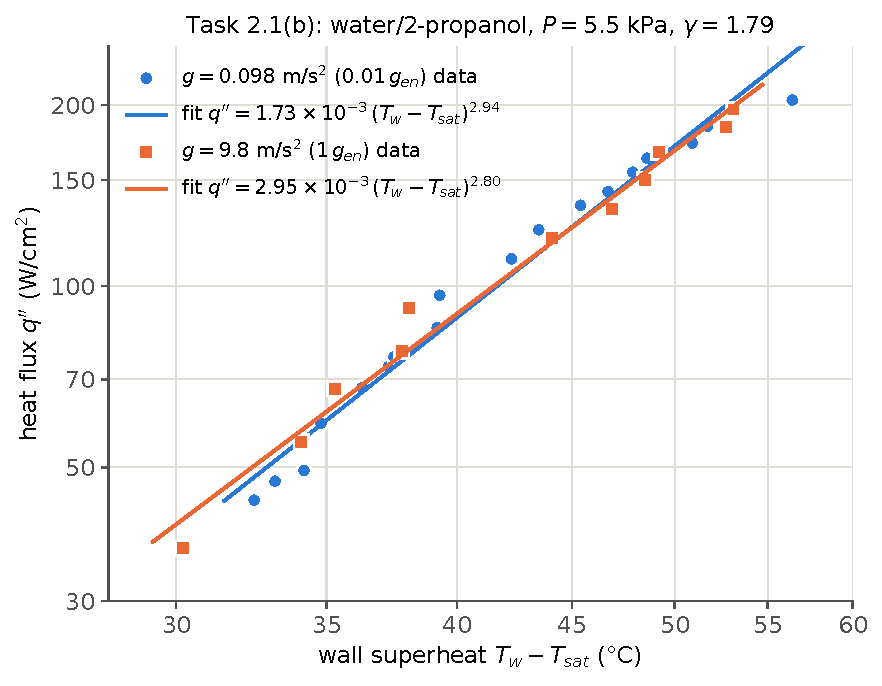
\includegraphics[width=0.66\linewidth]{figures/t21_loglog.pdf}
\caption{Task 2.1(b): heat flux versus wall superheat for $g=0.098$ and $9.8$~m/s$^2$ (log-log axes),
with a power-law fit for each gravity level.}
\label{fig:t21}
\end{figure}

% ---------------------------------------------------------------
\subsection{Task 2.2 -- Three-constant model $\qpp=n_1\dTsat^{n_2}g^{n_3}$}
\label{sec:t22}

\paragraph{Assembly of the program.}
\code{CodeP2.1F26} (data, corrected as above) and \code{CodeP2.2F26} were placed in two consecutive cells
of \code{P2\_Task2.2.ipynb}. \textbf{The program provided does not run as it is}: the line
\code{import random} at the top of \code{CodeP2.2F26} gives the name \code{random} to the
\emph{module} and hides the \emph{function} \code{random()} imported by \code{CodeP2.1F26}. The
initialisation \code{n1i+0.001*random()} then stops with
\code{TypeError: 'module' object is not callable}. I replaced it with \code{from random import random, seed}.
The other changes (Section~\ref{sec:codechanges}) do not modify the algorithm. The evolution loop is
placed in a function \code{run\_GA(n1i, n2i, n3i, NGEN, MUT, MFRAC, rseed)}, so that it can be re-run
for many initial guesses. The mutation amplitude (0.085 in the code) becomes the argument \code{MUT},
and both random generators are seeded.

\paragraph{First run (skeleton initial guesses).}
With the initial guesses of the skeleton ($n_1=0.00027$, $n_2=4.0$, $n_3=0.063$), MUT $=0.085$ and
NGEN $=6000$, $\Ferrmean$ drops below the target 0.035 after only \TwoTwoBaseKconv\ generations. The
minimum, $\Ferrmean=\TwoTwoBaseF$, is reached at generation \TwoTwoBaseKmin\ (first lines of
Table~\ref{tab:t22const}). The target is met. However, $n_2=3.34$ is far from the value
$n_2\approx3$ of Task~2.1(b), and a second look shows that this solution is not the best one.

\paragraph{Effect of the initial guesses, of the mutation amplitude and of NGEN.}
Four sets of initial guesses were tested (Table~\ref{tab:t22study}). Set~1 is the skeleton guess and
Set~2 a physics-based guess ($n_2=3$, $0.01<n_3<0.1$). Set~3 is far from the solution ($n_2=2$,
$n_3=0.25$) and Set~4 very far ($n_1$ about 1500 times too small, $n_2=5$). Each set was run with 5
different random seeds, for three maximum mutation amplitudes (MUT $=\pm8.5$, $\pm20$ and $\pm40\,\%$),
with a longer run (NGEN $=20000$), and with a two-stage strategy: exploration with MUT $=0.40$, then a
restart from the best constants with MUT $=0.03$. In total 88 runs were made.
Figure~\ref{fig:t22conv} shows the convergence histories and Figure~\ref{fig:t22land} the trajectories of
the population-average constants on the error landscape.

\begin{table}[H]
\centering\scriptsize
\caption{Task 2.2: effect of the initial guesses, of the maximum mutation amplitude MUT and of NGEN
(5 seeds per line, 2 for NGEN $=20000$). ``best/median/worst'' = minimum $\Ferrmean$ reached in a run;
``$<0.035$'' = number of runs that reach the target; $k_{0.035}$ = median generation at which the target is first
reached; last column = spread of the best-fit $n_2$ between seeds. Deterministic reference minimum:
$\Ferrmean=\TwoTwoRefF$ at $n_2=\TwoTwoRefNtwo$.}
\label{tab:t22study}
\fittable{t22_study}
\end{table}

\begin{figure}[H]
\centering
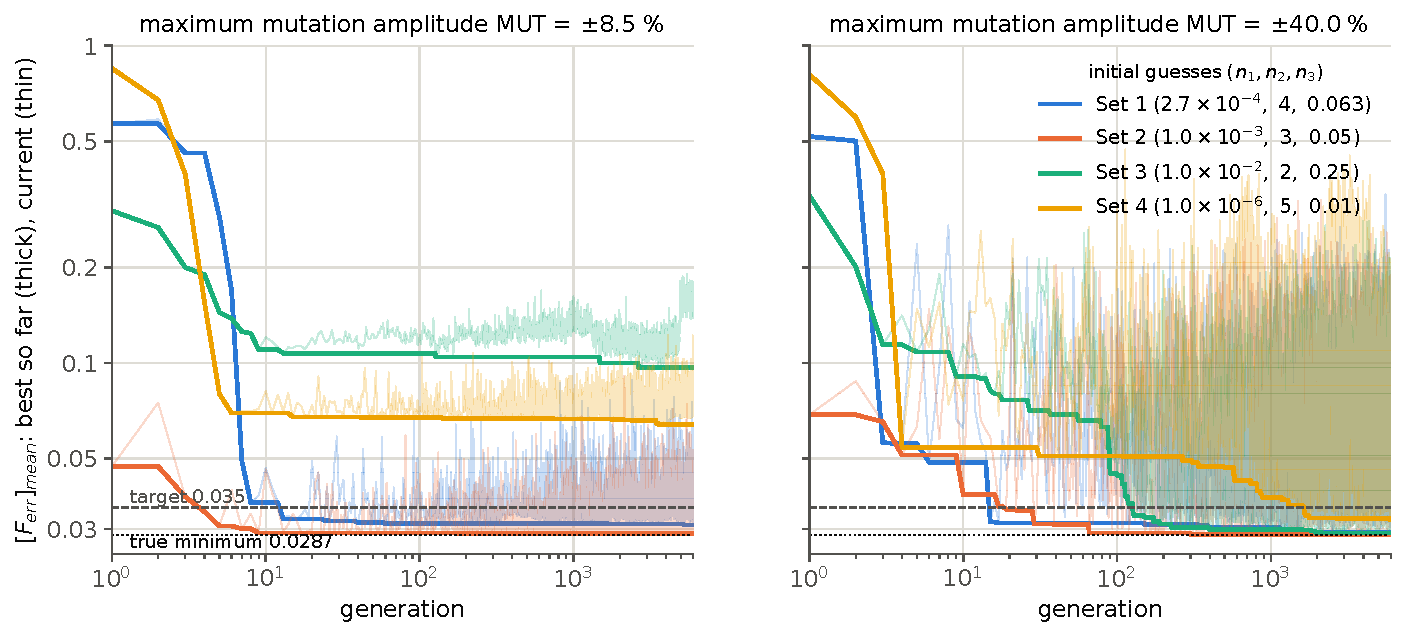
\includegraphics[width=\linewidth]{figures/t22_convergence.pdf}
\caption{Task 2.2: convergence of $\Ferrmean$ for the four sets of initial guesses (seed 1). Thick lines:
best value so far; thin lines: value at each generation. Left: skeleton mutation amplitude ($\pm8.5\,\%$);
right: $\pm40\,\%$.}
\label{fig:t22conv}
\end{figure}

\begin{figure}[H]
\centering
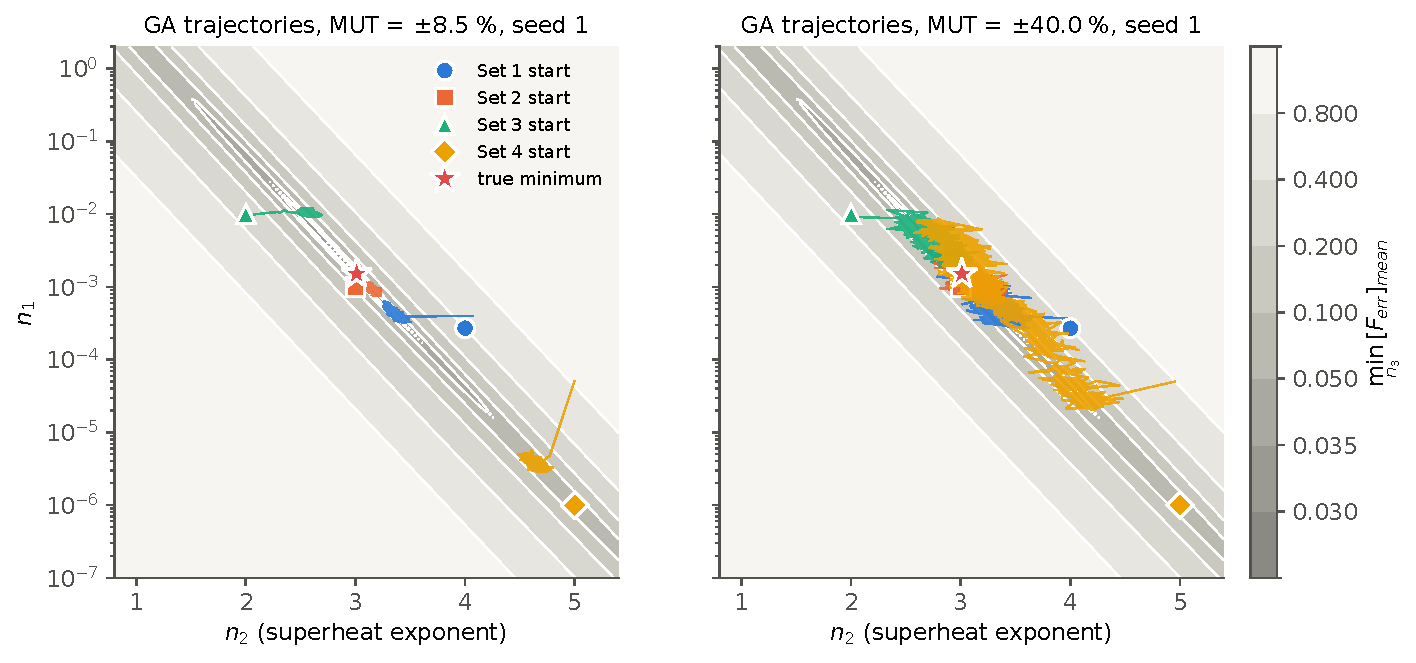
\includegraphics[width=\linewidth]{figures/t22_landscape.pdf}
\caption{Task 2.2: error landscape (minimum over $n_3$ of $\Ferrmean$ in the $(n_2,n_1)$ plane) and
trajectories of the population-average constants of the four sets (seed 1). The error has a long, narrow
valley along $\ln n_1+3.7\,n_2\approx\text{const}$.}
\label{fig:t22land}
\end{figure}

The main observations are:
\begin{itemize}
  \item \textbf{Guesses close to the solution (Sets 1 and 2) converge for every mutation amplitude and every
        seed}, in a few generations. The target 0.035 is reached after 2--12 generations, because the GA
        only has to adjust $n_1$ to the level of the data. Even so, with the skeleton amplitude
        ($\pm8.5\,\%$), Set~1 stops at $n_2=3.08$--$3.34$ depending on the seed. The error is below the target,
        but these constants are not the optimum.
  \item \textbf{The error surface is a narrow valley} (Fig.~\ref{fig:t22land}). Since
        $\ln\qpp=\ln n_1+n_2\ln\dTsat+n_3\ln g$ and $\ln\dTsat\approx3.7$ in the middle of the data,
        $\ln n_1$ and $n_2$ compensate each other: along the valley floor, $\Ferrmean$ stays below 0.035
        for $2.2\lesssim n_2\lesssim3.6$. A mutation of $\pm8.5\,\%$ on $n_2$ ($\pm0.26$) changes $\ln\qpp$
        by about $\pm1$, which is much more than the scatter of the data (about 0.15). As a result, almost only
        the offspring whose mutations of $n_1$ and $n_2$ compensate each other survive, and the population
        moves along the valley very slowly, like a random walk.
  \item \textbf{Far guesses (Sets 3 and 4) do not converge with the skeleton amplitude}, and giving
        them more generations does not help. With MUT $=0.085$, Set~3 reaches the target in only 1 run
        out of 5 and Set~4 never does. NGEN $=20000$ gives no improvement (0/2): the population remains trapped at $n_2\approx2.5$ with $n_3\approx0.2$
        (Set~3), or at $n_2\approx4.4$ (Set~4), with $\Ferrmean\approx0.06$--$0.10$. As suggested in the statement, \textbf{increasing the mutation
        amplitude solves the problem}. With $\pm40\,\%$, all runs of Sets~3 and 4 reach the target, after
        about 130 and 1600 generations. The cost is a much noisier population (thin lines in
        Fig.~\ref{fig:t22conv}), so the minimum is reached only occasionally.
  \item \textbf{The two-stage strategy (large mutations to explore, then small mutations to refine)
        combines robustness and accuracy.} It keeps the $100\,\%$ success rate of the $\pm40\,\%$ runs,
        even from Set~4. It lowers the median error of every set compared with the single $\pm40\,\%$ run,
        and it produced the overall best fit. For guesses that are already close to the solution, a
        moderate amplitude ($\pm20\,\%$) in a single run works just as well.
\end{itemize}

\paragraph{Best fit.}
The best of the 88 runs (\TwoTwoBestSet, two-stage, seed \TwoTwoBestSeed) gives the constants of
Table~\ref{tab:t22const}:
\[
\boxed{\qpp=\TwoTwoNone\,\dTsat^{\,\TwoTwoNtwo}\,g^{\,\TwoTwoNthree}}\qquad
\Ferrmean=\TwoTwoF\ (<0.035).
\]
This error is within $0.05\,\%$ of the true minimum of the error function ($\TwoTwoRefF$) found by the
deterministic check. The constants themselves differ slightly from the reference ($n_2$: $-1.2\,\%$,
$n_3$: $-6\,\%$, $n_1$: $+14\,\%$). This difference is the flat valley again: these sets of constants
describe the data equally well. The robust result is $n_2\approx3.0\pm0.05$ and a weak exponent
$n_3\approx0.045$.

\begin{table}[H]
\centering\small
\caption{Task 2.2: constants of Eq.~(1.1) printed by the program (MINIMUM = population-average constants
at the minimum of $\Ferrmean$, ENDING = last generation, TIME AVG = average over generations 801--NGEN).
$^\dagger$the TIME AVG error printed by the skeleton is the average of $\Ferrmean$ over all generations.}
\label{tab:t22const}
\fittable{t22_constants}
\end{table}

\paragraph{Predicted versus measured heat flux and rms deviation.}
Figure~\ref{fig:t22parity}(a) shows each pair $(\qpp_{pred},\qpp_{exp})$ as a discrete point on log-log
axes, with the line of slope 1 and the $\pm10\,\%$ lines. Figure~\ref{fig:t22parity}(b) shows the
fractional deviation for each gravity level. The deviation statistics are:
\begin{itemize}
  \item rms deviation of $\qpp_{exp}$ from $\qpp_{pred}$: $\TwoTwoRmsAbs$~W/cm$^2$ (mean heat flux
        $\TwoTwoMeanQ$~W/cm$^2$);
  \item rms fractional deviation $\sqrt{\overline{[(\qpp_{exp}-\qpp_{pred})/\qpp_{pred}]^2}}=\TwoTwoRmsRel\,\%$,
        mean absolute fractional deviation $\TwoTwoMeanAbsRel\,\%$, maximum $\TwoTwoMaxRel\,\%$;
  \item only $\TwoTwoWithin\,\%$ of the points are within $\pm10\,\%$ of the prediction.
\end{itemize}

\begin{figure}[H]
\centering
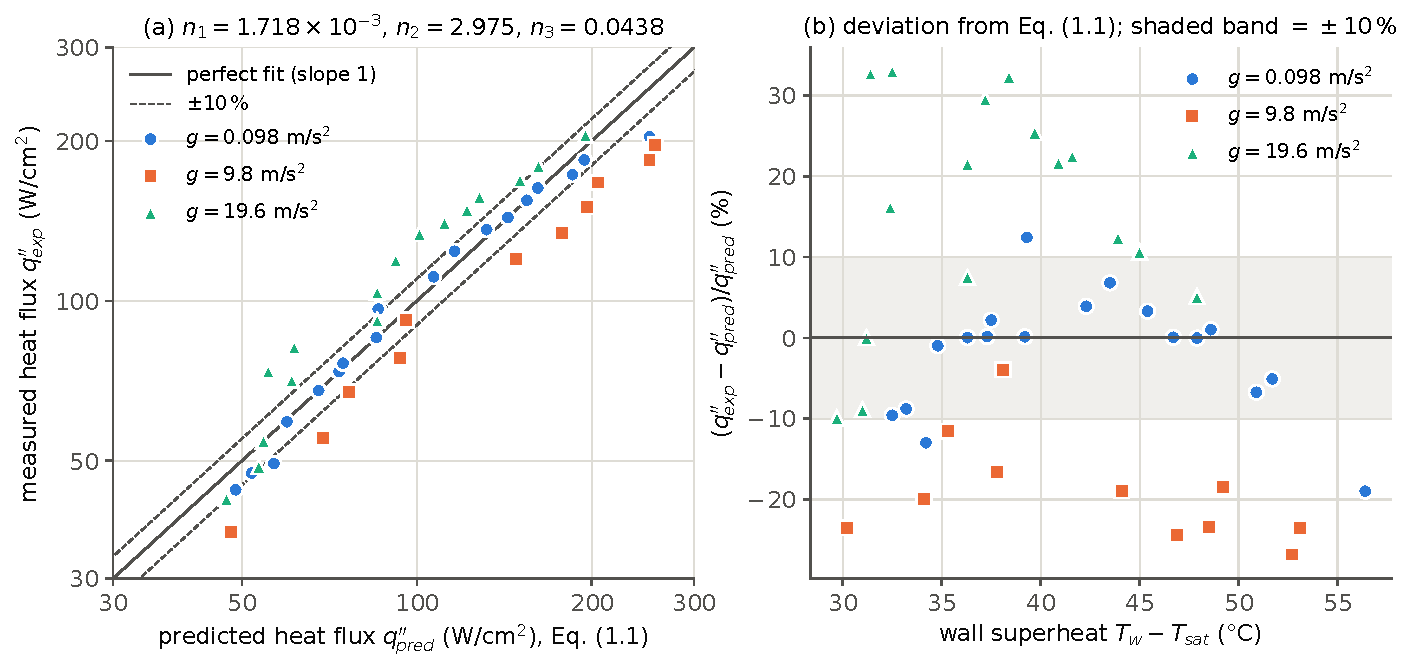
\includegraphics[width=\linewidth]{figures/t22_parity.pdf}
\caption{Task 2.2: (a) measured versus predicted heat flux for the best-fit constants (log-log); (b)
fractional deviation versus superheat. Each gravity level has its own symbol.}
\label{fig:t22parity}
\end{figure}

\paragraph{Assessment of the fit with respect to the $\pm10\,\%$ uncertainty.}
\textbf{The fit is not tighter than the uncertainty of the data}: the rms deviation ($\TwoTwoRmsRel\,\%$) and the
mean absolute deviation ($\TwoTwoMeanAbsRel\,\%$) are larger than the estimated $\pm10\,\%$
measurement uncertainty. The superheat is also uncertain: $\pm0.5$\,\textdegree C at 40\,\textdegree C gives $\pm4\,\%$ on
$\qpp$ through $n_2\approx3$, so the combined noise is about $10.7\,\%$. That is still clearly below the
rms deviation. \textbf{The deviation of the fit is therefore above the noise level of the data.} The
groups in Fig.~\ref{fig:t22parity}(b) show where it comes from. The deviations are
\emph{systematic}, not random:
\begin{center}\small
\begin{tabular}{@{}l c c@{}}
\toprule
Group & mean deviation & rms deviation\\
\midrule
$g=0.098$~m/s$^2$ (18 points) & $\TwoTwoBiasLow\,\%$  & $\TwoTwoRmsLow\,\%$\\
$g=9.8$~m/s$^2$ (11 points)   & $\TwoTwoBiasMid\,\%$  & $\TwoTwoRmsMid\,\%$\\
$g=19.6$~m/s$^2$ (16 points)  & $\TwoTwoBiasHigh\,\%$ & $\TwoTwoRmsHigh\,\%$\\
\bottomrule
\end{tabular}
\end{center}
The $0.01\,\gen$ group is fitted to within the noise ($7.5\,\%$ rms). The $1\,\gen$ group is overpredicted
by about $19\,\%$ and the $2\,\gen$ group underpredicted by about $16\,\%$. With a single exponent, $g^{n_3}$
cannot represent at the same time an almost zero change between $0.01$ and $1\,\gen$ (Task~2.1(b)) and a
$15$--$30\,\%$ increase between $1$ and $2\,\gen$, so $n_3$ ends up as a compromise. This is a
\textbf{model-form error}: the Marangoni contribution, which keeps the heat flux finite when $g\to0$, is
missing from Eq.~(1.1).

Consequences for the use of Eq.~(1.1):
\begin{itemize}
  \item \emph{Accuracy of the predictions}: a heat flux predicted by Eq.~(1.1) is uncertain by about
        $\pm17\,\%$ (one standard deviation), and up to $\pm30\,\%$ for some conditions. This is larger
        than the measurement uncertainty and depends on the gravity level (biased predictions at
        $1\,\gen$ and $2\,\gen$).
  \item \emph{Accuracy of the predicted trends}: the superheat trend ($n_2\approx3$) is robust. It agrees
        with Task~2.1(b) and changes little between the runs. The gravity trend is not reliable: the
        model predicts that $\qpp$ increases by $100^{n_3}-1\approx22\,\%$ between $0.01\,\gen$ and
        $1\,\gen$, while the data show almost no change. Extrapolating to $g\to0$ would even predict
        $\qpp\to0$, which is the opposite of the observed Marangoni behaviour.
  \item To bring the deviation down to the noise level, the model must contain the missing physics. The
        five-constant model of Task~2.3 adds it, and removes most (not all) of this bias.
\end{itemize}

% ---------------------------------------------------------------
\subsection{Task 2.3 -- Five-constant model $\qpp=n_1\dTsat^{n_2}(g+n_4\gen\gamma)^{n_3}P^{n_5}$}
\label{sec:t23}

\paragraph{Program.}
\code{P2\_Task2.3.ipynb} is a copy of the Task~2.2 program with modifications (i)--(vii) of the
statement (red data uncommented, $N_D=N_S=77$, error function Eq.~(1.7) in the two loops, mating of
$n_4$ and $n_5$, five-constant print-out and plot, initial guesses (vii)). They are listed in
Section~\ref{sec:codechanges}. I also added the 15 validation points of the Appendix (\code{vdata}).
They are never used by the GA; they only test the fitted relation on data it has not seen.

\paragraph{Run with the initial guesses (vii).}
The initial guesses of the statement already give $\Ferrmean=\TwoThreeFinit$. The GA (MUT $=\pm9\,\%$,
NGEN $=6000$) goes below the target 0.03 at generation \TwoThreeBaseKconv\ and reaches a minimum of
\TwoThreeBaseF\ at generation \TwoThreeBaseKmin\ (Table~\ref{tab:t23const}). The target is met. However,
the deterministic check shows that the error function can go down to \TwoThreeRefF, about $25\,\%$
lower, so a broader range of initial guesses was explored.

\paragraph{Range of initial guesses.}
Five sets of initial guesses were run with two mutation amplitudes and five seeds each
(Table~\ref{tab:t23study}):
(A)~the guesses (vii) of the statement;
(B)~no pressure effect ($n_5=0.01$) and the pure-fluid gravity exponent $n_3=0.25$;
(C)~stronger gravity/Marangoni and pressure effects ($n_3=n_5=0.5$, $n_4=2$);
(D)~a far guess;
(E)~all constants equal to 1.
The best single run of each seed was then refined in two more stages, restarted from its best constants
with MUT $=0.03$ and then $0.01$ (last column of Table~\ref{tab:t23study}).

\begin{table}[H]
\centering\scriptsize
\caption{Task 2.3: effect of the initial guesses (NGEN $=6000$, 5 seeds per line, 3 for MFRAC $=1$).
``frac.\ nkeep$=0$'' = fraction of generations without any survivor. ``refined'' = best and worst
$\Ferrmean$ after the two refinement stages (MUT $=0.03$ then $0.01$) for 3 seeds. Deterministic reference
minimum: $\TwoThreeRefF$.}
\label{tab:t23study}
\fittable{t23_study}
\end{table}

The behaviour is richer than for three constants:
\begin{itemize}
  \item \textbf{Set C converges almost immediately} (target reached in 2--3 generations, $\Ferrmean\approx0.022$),
        and its refinement gives the best fit, within $0.6\,\%$ of the true minimum.
  \item \textbf{Set A} (statement) always meets the target, but it stops at $0.025$--$0.030$, and at
        $0.022$--$0.023$ after refinement. It starts with $n_3\approx n_5\approx0.22$, on the wrong
        side of a long valley in the $(n_3,n_5)$ directions, and the population moves along this valley only
        slowly.
  \item \textbf{Set B shows a limitation of multiplicative mutations.} A constant guessed close to zero
        can hardly move: a $\pm9\,\%$ mutation of $n_5=0.01$ changes it by at most $\pm0.0009$. The
        pressure exponent therefore stays close to 0, the other constants have to compensate, and only
        3/10 runs reach the target. \emph{A constant whose sign or order of magnitude is unknown should not
        be initialised close to zero.}
  \item \textbf{Sets D and E fail}, even after refinement ($\Ferrmean\ge0.033$). With Set E and the skeleton
        settings, the population is even \emph{frozen}: in $90\,\%$ of the generations no organism has an
        error below $0.5\times$ median, so \code{nkeep}$\,=0$. All offspring are then mutations of the same
        organism \code{n[0]}, which is never replaced (the median error stays at 0.95). Larger mutations
        (MUT $=0.2$) or a less selective threshold (MFRAC $=1$) unfreeze the population, but 6000
        generations are not enough to reach the valley. The same mechanism is analysed in detail for
        Part~2 (Section~\ref{sec:part2}, Fig.~\ref{fig:t25nkeep}).
\end{itemize}

\paragraph{Best fit.}
The best-fit constants are given in Table~\ref{tab:t23const} (set \TwoThreeBestSet, seed \TwoThreeBestSeed, refined):
\[
\boxed{\qpp=\TwoThreeNone\,\dTsat^{\,\TwoThreeNtwo}\,\bigl(g+\TwoThreeNfour\,\gen\gamma\bigr)^{\TwoThreeNthree}\,P^{\,\TwoThreeNfive}}
\]
with $\Ferrmean=\TwoThreeF$ ($<0.03$) ($\qpp$ in W/cm$^2$, $T$ in \textdegree C, $g$ in m/s$^2$, $P$ in kPa). Figure~\ref{fig:t23evol} shows the evolution
of the constants and of the error. The deterministic check gives $\Ferrmean=\TwoThreeRefF$, with slightly
different constants ($n_2=\TwoThreeRefNtwo$, $n_3=\TwoThreeRefNthree$, $n_4=\TwoThreeRefNfour$,
$n_5=\TwoThreeRefNfive$). The profiles of Fig.~\ref{fig:t23prof} explain this difference. When one
constant is fixed and the four others are re-optimised, the minimum error increases by only $3\,\%$ (to
about 0.0215) over the ranges $n_2\approx2.8$--$3.2$ ($\pm7\,\%$), $n_3\approx0.41$--$0.54$
($\pm14\,\%$), $n_4\approx1.1$--$1.65$ ($\pm20\,\%$) and $n_5\approx0.28$--$0.65$ ($\pm40\,\%$).
The superheat exponent is therefore well determined by the data, $n_3$ reasonably well, and $n_4$ and
$n_5$ only weakly. Constants with this kind of uncertainty can differ between equally good fits. This is
expected for $n_5$: pressures other than 5.5~kPa appear only in two groups, and the 7.0~kPa group is
also the only one with $\gamma=0$.

\begin{table}[H]
\centering\scriptsize
\caption{Task 2.3: constants of Eq.~(1.5). $^\dagger$average of $\Ferrmean$ over all generations.}
\label{tab:t23const}
\fittable{t23_constants}
\end{table}

\begin{figure}[H]
\centering
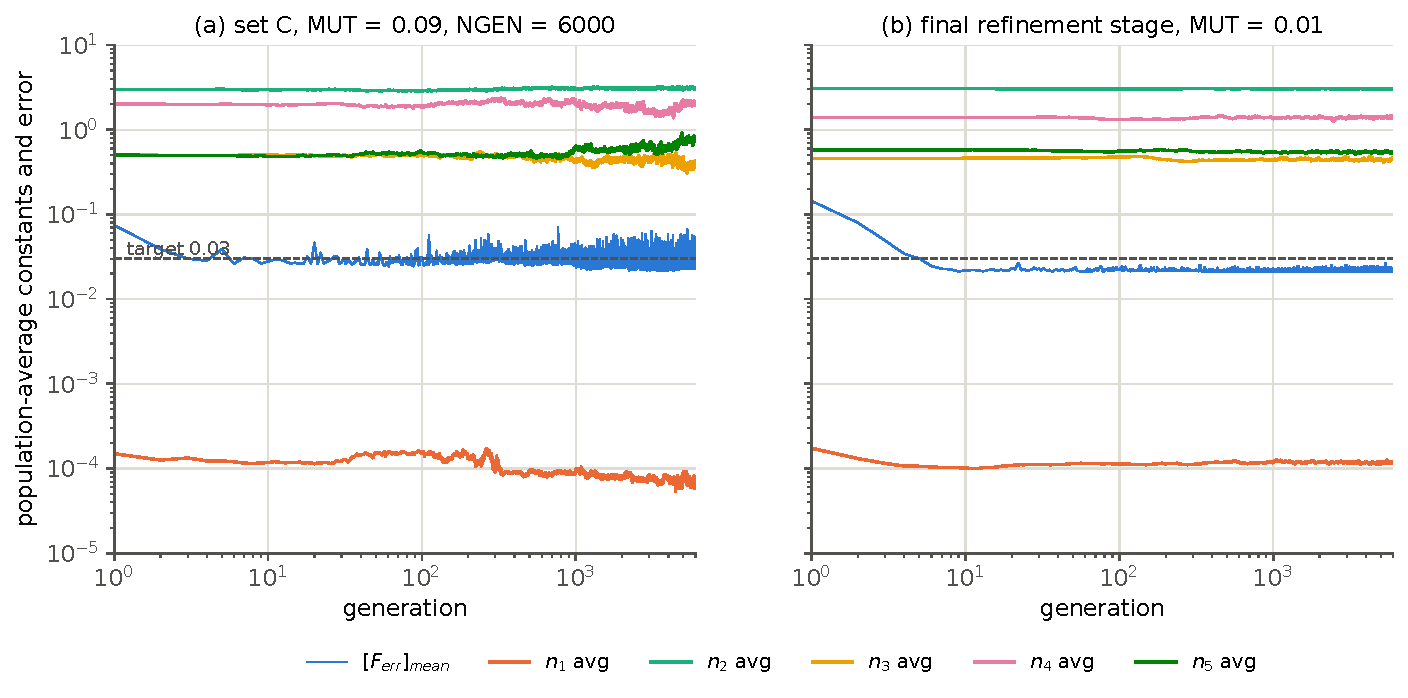
\includegraphics[width=\linewidth]{figures/t23_evolution.pdf}
\caption{Task 2.3: population-average constants and error of the best-fit sequence. (a) Main GA run from
set C; (b) last refinement stage (MUT $=0.01$).}
\label{fig:t23evol}
\end{figure}

\begin{figure}[H]
\centering
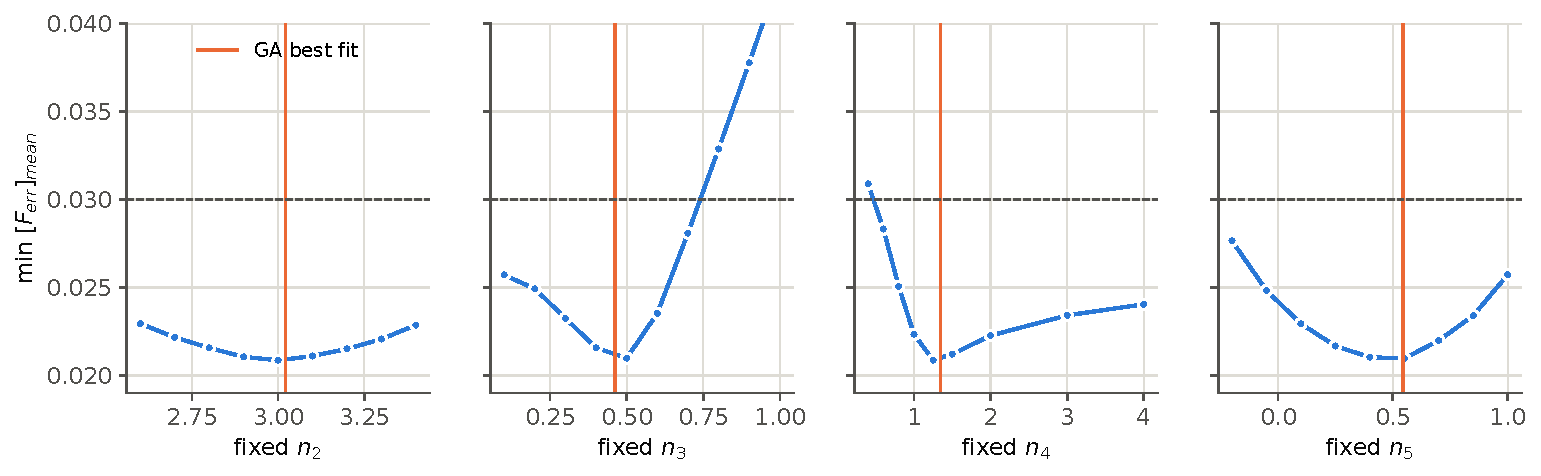
\includegraphics[width=\linewidth]{figures/t23_profiles.pdf}
\caption{Task 2.3: minimum achievable $\Ferrmean$ when one constant is fixed and the four others are
re-optimised. A flat profile means that the data determine this constant only weakly.}
\label{fig:t23prof}
\end{figure}

\paragraph{Quality of the fit and validation.}
Figure~\ref{fig:t23parity} compares the predictions with the 77 training points and the 15
validation points.
\begin{itemize}
  \item Training data: rms fractional deviation $\TwoThreeRmsTrain\,\%$, mean absolute deviation
        $\TwoThreeMadTrain\,\%$, $\TwoThreeWithinTrain\,\%$ of the points within $\pm10\,\%$. For the
        45 points of Task~2.2, the three-constant model gave $16.6\,\%$, $13.2\,\%$ and $47\,\%$.
  \item Validation data: $\Ferrmean=\TwoThreeFval$, rms fractional deviation $\TwoThreeRmsVal\,\%$, mean
        absolute deviation $\TwoThreeMadVal\,\%$.
\end{itemize}
Overall, the deviation is now close to the estimated noise of the data (about $10$--$11\,\%$). The
validation error is only slightly larger than the training error, so the five-constant model does not
over-fit (77 points for 5 constants). The largest validation deviation is the point
$(\qpp,T_w-T_{sat})=(50.9,\ 37.2)$ at $0.01\,\gen$: its superheat is 3\,\textdegree C higher than that of the
training point with almost the same heat flux ($49.4$~W/cm$^2$ at $34.2$\,\textdegree C), which points to measurement scatter.

\textbf{The remaining deviation is not entirely random, however.} Table~\ref{tab:t23bias} gives the mean
deviation of each test condition. Four conditions are fitted within the noise (mean deviation between
$\TwoThreeBiasOthersMin\,\%$ and $\TwoThreeBiasOthersMax\,\%$). Two are still biased: the $1\,\gen$ group
is overpredicted by about $16\,\%$ (mean deviation $\TwoThreeBiasOneG\,\%$) and the $2\,\gen$ group at 5.5~kPa is
underpredicted by about $11\,\%$ (mean deviation $\TwoThreeBiasTwoG\,\%$). The equivalent-gravity term reduces the
gravity bias of Eq.~(1.1) ($-19\,\%$ and $+16\,\%$ for the same two groups) but does not remove it.
With a single exponent $n_3$, the form $(g+n_4\gen\gamma)^{n_3}$ cannot give at the same time almost no
change between $0.01$ and $1\,\gen$ and a $40$--$50\,\%$ increase between $1$ and $2\,\gen$ at 5.5~kPa
(Fig.~\ref{fig:t23parity}). Part of the gravity effect is therefore still missing from Eq.~(1.5), and
predictions at $1$ and $2\,\gen$ carry this systematic error on top of the scatter.

\begin{table}[H]
\centering\small
\caption{Task 2.3: mean and rms deviation $(\qpp_{exp}-\qpp_{pred})/\qpp_{pred}$ for each test condition
(training data). Mean deviations larger than $10\,\%$ are in bold. Last column: the three-constant fit
of Task~2.2 for the groups it was fitted on.}
\label{tab:t23bias}
\fittable{t23_bias}
\end{table}

\begin{figure}[H]
\centering
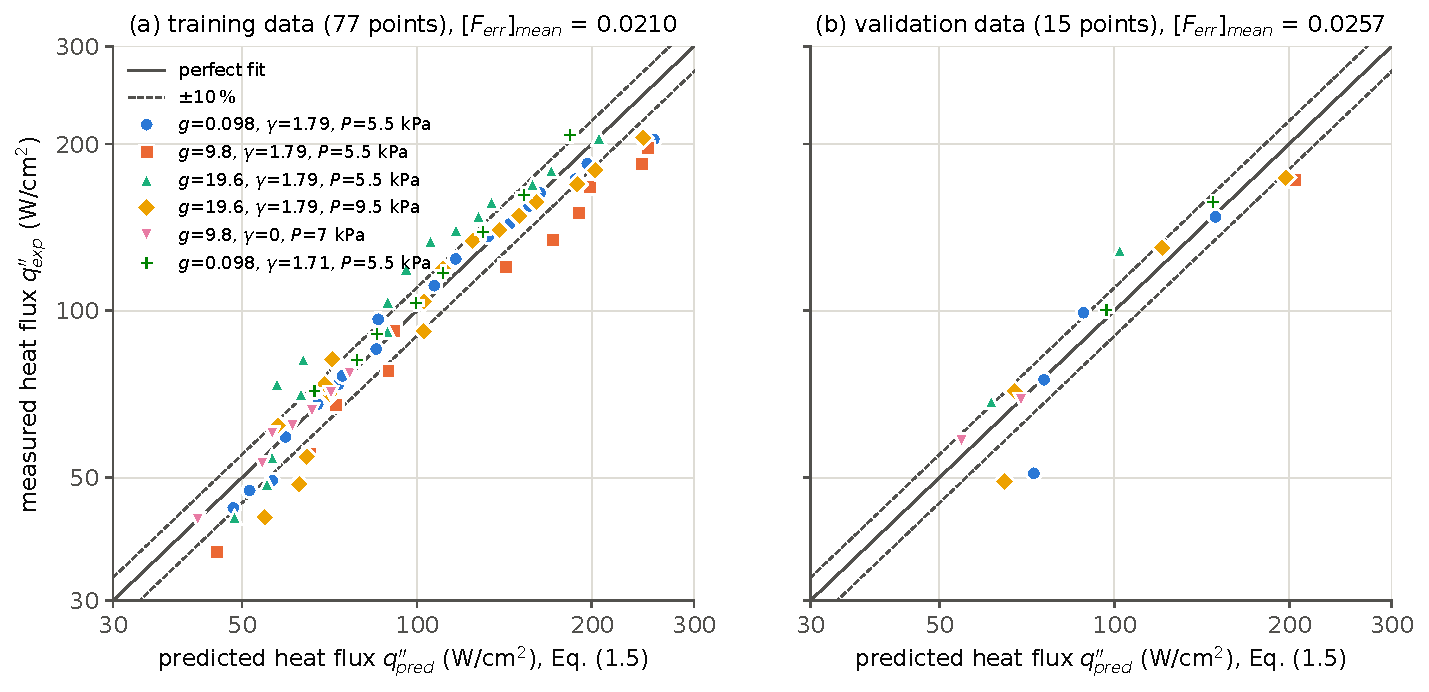
\includegraphics[width=\linewidth]{figures/t23_parity.pdf}
\caption{Task 2.3: measured versus predicted heat flux, Eq.~(1.5) with the best-fit constants. (a) 77
training points; (b) 15 validation points. One symbol per test condition.}
\label{fig:t23parity}
\end{figure}

\paragraph{Surface plot and physical interpretation.}
Figure~\ref{fig:t23surf} shows $\qpp/\dTsat^{n_2}=n_1(g+n_4\gen\gamma)^{n_3}P^{n_5}$ for
$1<g<20$~m/s$^2$ and $0<\gamma<2$ at $P=10$~kPa. Three conclusions follow:
\begin{itemize}
  \item \textbf{The Marangoni effect acts like an additional gravity.} The term $n_4\gen\gamma$ is an
        ``equivalent gravity'' produced by the surface tension gradients. For $\gamma=1.79$ it equals
        $\TwoThreeGeq$~m/s$^2$ ($\approx\TwoThreeGeqRatio\,\gen$), which is larger than earth gravity. This is
        why $\qpp$ depends so little on gravity at low $g$: between $0.01\,\gen$ and $1\,\gen$ the effective
        gravity only goes from about 24 to 33~m/s$^2$. The model still predicts $+17\,\%$ over this range,
        where the data show almost no change (Task~2.1(b)); this is the residual bias of Table~\ref{tab:t23bias}.
  \item \textbf{The gravity dependence depends on $\gamma$.} Without Marangoni effect ($\gamma=0$),
        $\qpp/\dTsat^{n_2}$ increases by a factor of 4 between $g=1$ and $20$~m/s$^2$. For $\gamma=2$ it
        increases by only $27\,\%$. At $g=1$~m/s$^2$, going from $\gamma=0$ to $\gamma=2$ multiplies the
        heat flux by 4.6. This is why a mixture with a positive $\gamma$ is attractive for low-gravity
        applications.
  \item The superheat exponent $n_2\approx3.0$ agrees with Tasks~2.1(b) and 2.2. The positive pressure
        exponent ($n_5\approx0.5$) agrees with the known increase of nucleate boiling heat transfer with
        pressure (through the fluid properties).
\end{itemize}

\begin{figure}[H]
\centering
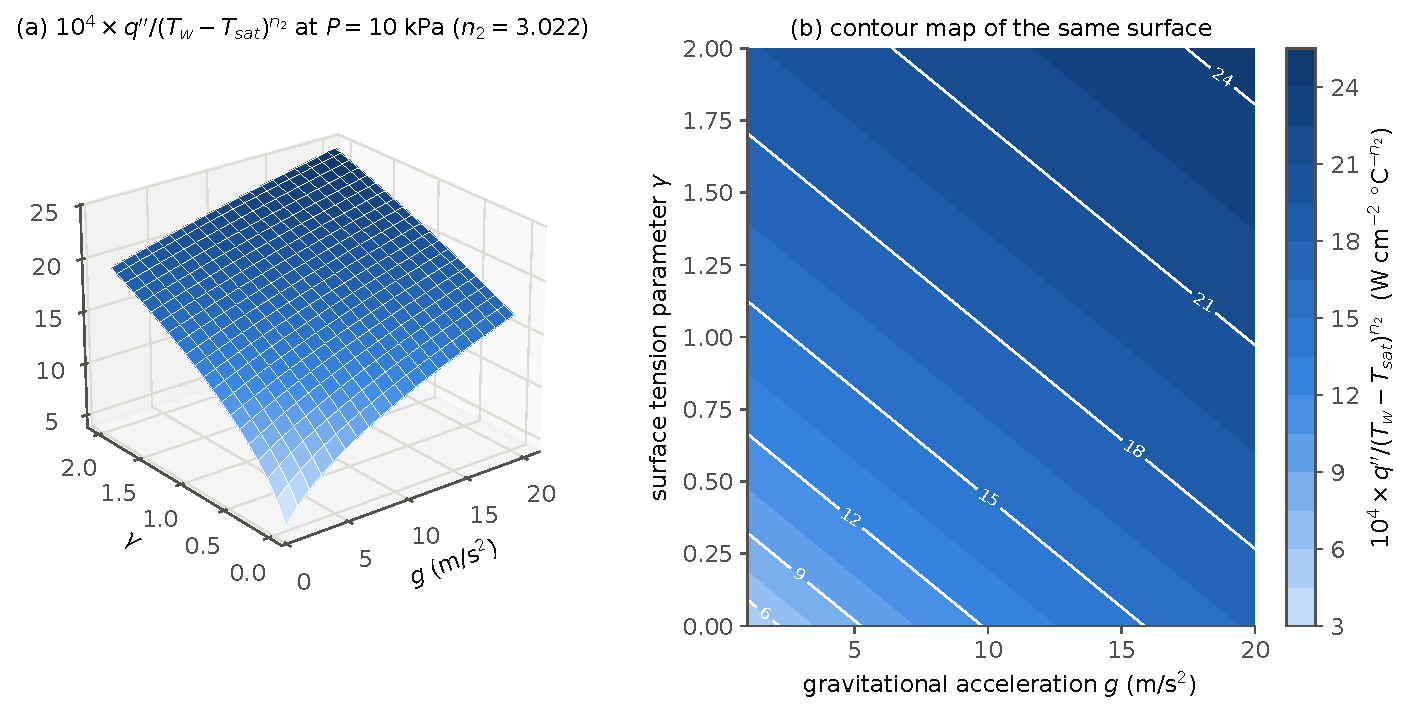
\includegraphics[width=\linewidth]{figures/t23_surface.pdf}
\caption{Task 2.3: $\qpp/\dTsat^{n_2}$ versus $g$ and $\gamma$ at $P=10$~kPa for the best-fit constants:
(a) surface plot; (b) contour map of the same surface.}
\label{fig:t23surf}
\end{figure}

% ---------------------------------------------------------------
\subsection{Extra Task ET1 -- Fractional sensitivity of the heat flux to the inputs}
\label{sec:et1}

\paragraph{Method.}
Program \code{P2\_ET1.ipynb} uses the best-fit constants of Task~2.3 and follows steps 1--3 of the
statement for three typical sets of inputs: S1 (earth gravity, $\dTsat_1=40$\,\textdegree C, $g_1=9.8$~m/s$^2$,
$\gamma_1=1.79$, $P_1=5.5$~kPa), S2 (the same at $0.01\,\gen$) and S3 ($2\,\gen$, 9.5~kPa, 35\,\textdegree C).
\begin{enumerate}[label=\arabic*)]
  \item $\qpp_1$ is computed with Eq.~(1.5) for the typical inputs;
  \item one input at a time is changed: the superheat by $\Delta\dTsat=2$\,\textdegree C, as in the statement, and
        $g$, $\gamma$, $P$ by $5\,\%$ (the same relative step as 2\,\textdegree C at 40\,\textdegree C), giving $\qpp_2$;
  \item the fractional change ratio is
        $S_x=\dfrac{\Delta\qpp/\qpp_1}{\Delta x/x_1}=\dfrac{(\qpp_2-\qpp_1)\,x_1}{\Delta x\,\qpp_1}$.
\end{enumerate}
For comparison, the limit $\Delta x\to0$ gives analytical values: $S_{T}=n_2$,
$S_g=n_3\,g/(g+n_4\gen\gamma)$, $S_\gamma=n_3\,n_4\gen\gamma/(g+n_4\gen\gamma)$ and $S_P=n_5$.

\begin{table}[H]
\centering\small
\caption{ET1: fractional change ratios (finite steps). The analytical limit $\Delta x\to0$ is given in
parentheses.}
\label{tab:et1}
\fittable{et1_sens}
\end{table}

\begin{figure}[H]
\centering
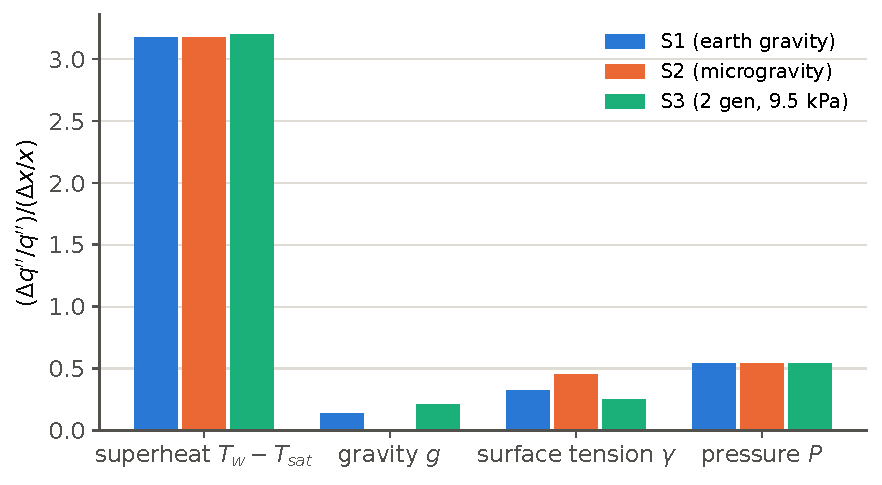
\includegraphics[width=0.62\linewidth]{figures/et1_sensitivity.pdf}
\caption{ET1: fractional sensitivity of the predicted heat flux to each input for the three typical states.}
\label{fig:et1}
\end{figure}

\paragraph{Results (Table~\ref{tab:et1}, Fig.~\ref{fig:et1}).}
\begin{itemize}
  \item \textbf{The heat flux is by far most sensitive to the superheat}: $S_T=\EtOneSdT$. A $1\,\%$ error
        on $T_w-T_{sat}$ gives a $3\,\%$ error on $\qpp$. The finite-step value is a little higher than
        $n_2=3.02$ because $(1.05)^{3.02}-1=0.159$ is more than $3.02\times0.05$ (non-linearity of the
        power law).
  \item The sensitivity to pressure is the same in all states ($S_P\approx n_5\approx0.54$).
  \item The sensitivities to $g$ and $\gamma$ depend on the state, because the two effects share the
        effective gravity $g+n_4\gen\gamma$. At earth gravity, $S_g=\EtOneSg$ and $S_\gamma=\EtOneSgam$.
        In microgravity, $S_g=\EtOneSgLow$: the gravity level no longer matters, and $S_\gamma$ increases
        to \EtOneSgamLow\ because Marangoni flow provides almost all the liquid supply.
\end{itemize}

\paragraph{Limiting fractional inaccuracy of the inputs for $|\Delta\qpp/\qpp|<0.15$.}
To first order,
$\Delta\qpp/\qpp=S_T\,\varepsilon_T+S_g\,\varepsilon_g+S_\gamma\,\varepsilon_\gamma+S_P\,\varepsilon_P$, where
$\varepsilon_x=\Delta x/x$. Three estimates are given in Table~\ref{tab:et1lim}:
(i) only one input is inaccurate, $\varepsilon_x<0.15/|S_x|$;
(ii) all inputs have the same inaccuracy $\varepsilon$ and the errors add up in the worst direction,
$\varepsilon<0.15/\sum|S_x|$;
(iii) the same $\varepsilon$, but independent random errors combined as a root-sum-square,
$\varepsilon<0.15/\sqrt{\sum S_x^2}$.

\begin{table}[H]
\centering\small
\caption{ET1: limiting fractional inaccuracy of the inputs for a fractional inaccuracy of the predicted
heat flux below 0.15. Last column: corresponding superheat uncertainty for case (ii).}
\label{tab:et1lim}
\fittable{et1_limits}
\end{table}

\textbf{Conclusion.} The superheat must be known to about $\EtOneSingle\,\%$ if it is the only
inaccurate input ($\pm\EtOneSingleC$\,\textdegree C at 40\,\textdegree C). If all inputs have the same fractional inaccuracy
and the errors add up, they must all be known to about $\EtOneWorst\,\%$ ($\pm\EtOneWorstC$\,\textdegree C on the
superheat). With random, independent errors the limit is about $\EtOneRss\,\%$. These estimates were
checked with the full non-linear model: changing all inputs by $3.6\,\%$ in the unfavourable direction
gives $\Delta\qpp/\qpp=\EtOneCheck\,\%$. Since the superheat dominates, a practical error budget is, for
example, superheat $\pm3\,\%$ ($\pm1.2$\,\textdegree C), pressure $\pm3\,\%$, $\gamma$ $\pm5\,\%$ and $g$ $\pm10\,\%$.
Even in the worst case, this gives $3.18(0.03)+0.54(0.03)+0.32(0.05)+0.13(0.10)=0.14<0.15$.
\textbf{The accuracy of the predicted heat flux is therefore limited mainly by the accuracy of the wall
superheat measurement.} An uncertainty of $\pm2$\,\textdegree C, which is not unusual for a wall temperature
measurement in a flight experiment, would by itself use up the whole $15\,\%$ budget.

% ---------------------------------------------------------------
\subsection{Extra Task ET2 -- Inverse relation for the superheat}
\label{sec:et2}

\paragraph{Method.}
Program \code{P2\_ET2.ipynb} reorganises the 77 data points of Task~2.3 as
$[T_w-T_{sat},\ \qpp,\ g,\ \gamma,\ P]$, so that $\qpp$, $g$, $\gamma$, $P$ are the inputs and the
superheat is the output. It then fits Eq.~(ET2.1),
$\dTsat=\nh1(\qpp)^{\nh2}(g+\nh4\gen\gamma)^{\nh3}P^{\nh5}$, with a copy of the Task~2.3 GA (error
normalised by $|\ln\dTsat|$). Three sets of initial guesses were used: (I) the values implied by Task~2.3,
(II) $(10,\,0.5,\,-0.1,\,1,\,-0.1)$ and (III) $(40,\,0.25,\,-0.25,\,2,\,-0.3)$, each with 3 seeds and the
same refinement as in Task~2.3. The best GA fit is
$\dTsat=20.27\,(\qpp)^{0.3074}(g+1.308\,\gen\gamma)^{-0.1455}P^{-0.1485}$ with $\Ferrmean=\EtTwoGaF$.
The superheat is predicted with an rms deviation of 1.8\,\textdegree C (mean absolute deviation $3\,\%$, about one
third of the deviation on $\qpp$, consistent with $n_2\approx3$).

\begin{table}[H]
\centering\small
\caption{ET2: best-fit $\hat n_i$ from the GA fit of (ET2.1), compared with the values computed from
the best-fit $n_i$ of Task~2.3 with the relations of the statement. Right: the same comparison between the
exact minima of the two error functions (deterministic check). Difference $=(\text{fit}-\text{implied})/|\text{implied}|$;
for the negative exponents $\hat n_3$ and $\hat n_5$, a positive difference means a smaller magnitude.}
\label{tab:et2}
\fittable{et2_table}
\end{table}

\paragraph{Do the two sets of $\hat n_i$ agree?}
They are \emph{close but not identical} (Table~\ref{tab:et2}). The differences are typically
$3$--$10\,\%$: $\nh1$ $\EtTwoDiffOne\,\%$, $\nh2$ $\EtTwoDiffTwo\,\%$, $\nh3$ $\EtTwoDiffThree\,\%$, $\nh4$
$\EtTwoDiffFour\,\%$, and up to $\EtTwoDiffFive\,\%$ for the weakly determined pressure exponent $\nh5$. The
only systematic difference is on $\nh2$: the direct fit of the superheat gives an exponent on $\qpp$
about $7$--$8\,\%$ smaller than $1/n_2$. The same differences appear between the exact minima of the two
error functions (right part of the table), so they are not caused by the GA. The implied values also give a
larger error for (ET2.1) ($\EtTwoImpF$ vs.\ $\EtTwoGaF$), which shows that the two fits really are different
optima.

\paragraph{Is the noise in the data responsible?}
Yes. Fitting $y$ versus $x$ and $x$ versus $y$ gives two slopes whose product is $r^2<1$ when the data
scatter, so the inverse exponent $\nh2$ must come out smaller than $1/n_2$. To check this quantitatively,
I made synthetic data with Eq.~(1.5) and the Task~2.3 constants, at the 77 measured conditions
(Table~\ref{tab:et2noise}):
\begin{itemize}
  \item[(a)] \textbf{Noise-free data}: the GA fit of (ET2.1) ($\Ferrmean=\EtTwoNoiseFreeF$) recovers the
        implied values to within $0.03\,\%$. The method and the relations of the statement are therefore
        exact when there is no noise.
  \item[(b)] \textbf{Scatter added to $\qpp$} (log-normal, standard deviation $\EtTwoSigma$, equal to the
        rms residual of the Task~2.3 fit; 30 realisations): the inverse fit gives $\nh2$ $7\pm2\,\%$ below
        $1/n_2$, exactly the difference found with the measured data. The other exponents scatter by
        $\pm5$--$10\,\%$ from one realisation to the next, which is the size of the differences in
        Table~\ref{tab:et2}.
  \item[(c)] \textbf{The same scatter put on the superheat instead} gives the same result. Which variable
        carries the noise only changes which of the two fits is unbiased, not the fact that they disagree.
\end{itemize}

\begin{table}[H]
\centering\small
\caption{ET2: percentage difference between the inverse fit and the values implied by the forward fit,
for the measured data and for synthetic data generated with Eq.~(1.5) (mean $\pm$ standard deviation over
30 noise realisations).}
\label{tab:et2noise}
\fittable{et2_noise}
\end{table}

\textbf{Conclusion.} The differences between the directly fitted $\hat n_i$ and those computed from
the Task~2.3 constants ($\approx2$--$17\,\%$, typically $5$--$10\,\%$) come from the scatter in the data:
it produces a systematic $\approx7\,\%$ reduction of $\nh2$ (regression dilution) and random differences of
the other constants of the same size as their run-to-run variability. The two relations are equally valid
descriptions of the data. Each one should be used in the direction in which it was fitted: the heat flux
from the superheat with Eq.~(1.5), and the superheat from the heat flux with Eq.~(ET2.1).

\begin{figure}[H]
\centering
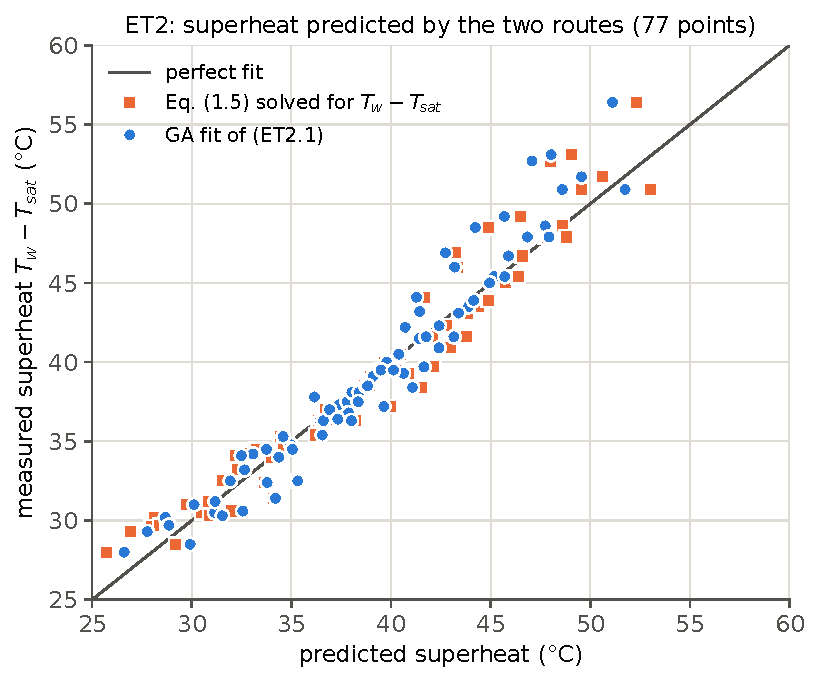
\includegraphics[width=0.55\linewidth]{figures/et2_parity.pdf}
\caption{ET2: measured superheat versus the superheat predicted by the GA fit of (ET2.1) and by Eq.~(1.5)
solved for $T_w-T_{sat}$.}
\label{fig:et2}
\end{figure}

% ===============================================================
\section{Part 2 -- Heat-pipe heat exchanger for an electronics cabinet}
\label{sec:part2}
% ===============================================================

\subsection{Task 2.4 -- Genetic algorithm program for the heat-pipe model}
\label{sec:t24}

\paragraph{Model.}
Equation~(2.3) can be written as two thermal conductances in series:
\begin{equation}
\dot q=\frac{T_{a,in}-T_{a,out}}{\dfrac{1}{(UA)_e}+\dfrac{1}{(UA)_c\left(1+\alpha\,h_r/h_{c,ref}\right)}},\qquad
h_r=\sigma\,(T_{a,in}+T_{a,out})(T_{a,in}^2+T_{a,out}^2),
\label{eq:hp}
\end{equation}
with absolute temperatures in $h_r$, $\sigma=5.67\times10^{-8}$~W\,m$^{-2}$K$^{-4}$ and
$h_{c,ref}=80$~W\,m$^{-2}$K$^{-1}$. Over the range of the data, $h_r$ varies only between 5.8 and
7.2~W\,m$^{-2}$K$^{-1}$, i.e.\ $h_r/h_{c,ref}=0.073$--$0.090$. The radiation correction is therefore a
small, slowly varying term. As in the statement, $n_1=(UA)_e$, $n_2=(UA)_c$ and $n_3=\alpha$.

\paragraph{Program and data.}
\code{P2\_Task2.4-2.5.ipynb} is a copy of the Task~2.2 program (modifications listed in
Section~\ref{sec:codechanges}). The 122 data points of \code{CodeP2.3F26} were split at random, with a
fixed seed, into a \textbf{training set of 98 points ($80.3\,\%$)} and a \textbf{validation set of 24
points ($19.7\,\%$)}. The GA uses only the training set ($N_S=N_D=98$). The error function is the
fractional error of the heat transfer rate, Eqs.~(2.4)--(2.5). It is coded once in \code{qdot\_model()}
(Eq.~(2.6)) and used in the two locations of the code (fitness loop and population-average loop) and in the
plots. The mean absolute error (MAE) of the validation set is computed at each generation with the
population-average constants, for monitoring only.

\subsection{Task 2.5 -- Results}
\label{sec:t25}

\paragraph{Initial guesses of order one.}
Following the statement, four sets of positive initial guesses of order one were used:
Set~1 $(1,1,1)$, Set~2 $(2,2,0.5)$, Set~3 $(5,5,1)$ and Set~4 $(10,3,2)$. Each set was run with the
skeleton selection (MFRAC $=0.5$) and two mutation amplitudes ($\pm9\,\%$, $\pm30\,\%$), and with
MFRAC $=1.0$, with 3 seeds each and NGEN $=6000$ (Table~\ref{tab:t25study}).

\begin{table}[H]
\centering\scriptsize
\caption{Task 2.5: effect of the initial guesses, of the mutation amplitude and of the selection fraction
MFRAC (NGEN $=6000$, 3 seeds per line). MAE = mean absolute fractional error, Eq.~(2.5)/$N_D$. ``valid.\ MAE''
is the MAE of the validation set for the best run. ``frac.\ nkeep$=0$'' = fraction of generations without any
survivor.}
\label{tab:t25study}
\fittable{t25_study}
\end{table}

\begin{figure}[H]
\centering
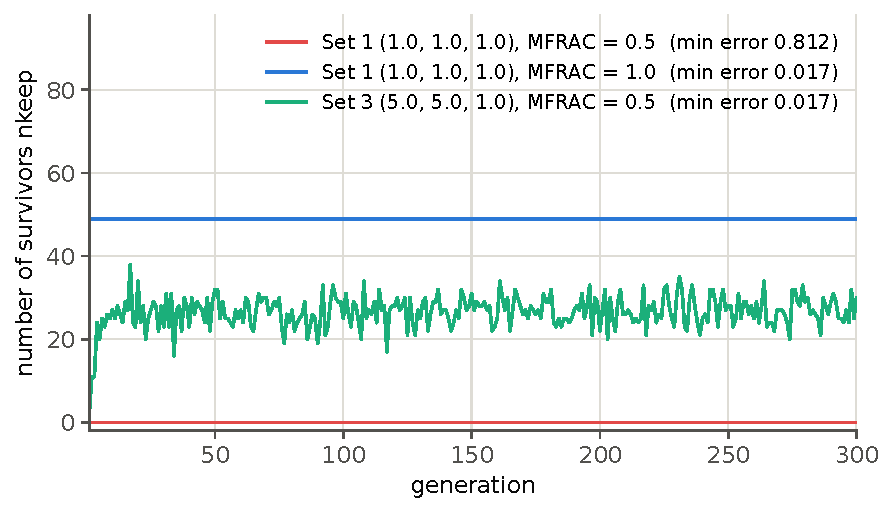
\includegraphics[width=0.66\linewidth]{figures/t25_nkeep.pdf}
\caption{Task 2.5: number of survivors per generation. With $(1,1,1)$ and the skeleton threshold
(MFRAC $=0.5$) no organism ever survives and the population is frozen. With MFRAC $=1$, half of the
population survives at every generation.}
\label{fig:t25nkeep}
\end{figure}

\begin{itemize}
  \item \textbf{Sets 3 and 4 converge immediately.} Their initial effective conductance is already
        close to the data ($\dot q/(T_{a,in}-T_{a,out})\approx2.9$~W/\textdegree C). The target 0.045 is reached in
        2--6 generations, and all runs end at a training MAE of 0.0166--0.0167.
  \item \textbf{Sets 1 and 2 do not converge at all with the skeleton algorithm, whatever the mutation
        amplitude.} The error stays at its initial value (0.81 and 0.64). Figure~\ref{fig:t25nkeep} and
        the column ``nkeep$=0$'' show why. With $(1,1,1)$, every organism predicts a heat transfer rate
        about 5 times too small, so all the fractional errors are close to $0.81$ with a very small spread.
        No error is below $0.5\times$ median, so \code{nkeep}$\,=0$ at \emph{every} generation. The
        offspring are then all mutations of organism \code{n[0]}, and this organism is never replaced
        (offspring are stored from index \code{nkeep+1}). Each generation is a new random cloud around the
        same frozen parent, nothing accumulates, and a larger mutation amplitude does not help.
  \item \textbf{With MFRAC $=1$} (the organisms with an error below the median survive), half of the
        population survives at every generation. Sets 1 and 2 then converge (target reached after 84 and 55
        generations) to the same error as Sets 3 and 4. Changing a single selection parameter turns a
        frozen algorithm into a robust one.
\end{itemize}

\paragraph{Effect of the number of generations.}
Table~\ref{tab:t25ngen} shows that, once the population is in the right region, NGEN has almost no effect.
From $(5,5,1)$, 100 generations already give the final error. From $(1,1,1)$ with MFRAC $=1$, about
500--2000 generations are needed. More generations do not lower the validation error either (no
over-fitting with only 3 constants): once converged, it stays between 0.0204 and 0.0208.

\begin{table}[H]
\centering\small
\caption{Task 2.5: effect of NGEN (range over 3 seeds; MUT $=\pm9\,\%$).}
\label{tab:t25ngen}
\fittable{t25_ngen}
\end{table}

\paragraph{Best fit.}
The best run (lowest \emph{training} error; the validation set was not used to select it) is
\TwoFiveBestSet\ $(5,5,1)$ with NGEN $=\TwoFiveBestNgen$ (seed \TwoFiveBestSeed):
\begin{center}
\begin{tabular}{@{}l c@{}}
\toprule
$n_1=(UA)_e$ & \TwoFiveNone~W/\textdegree C\\
$n_2=(UA)_c$ & \TwoFiveNtwo~W/\textdegree C\\
$n_3=\alpha$ & \TwoFiveNthree\\
\midrule
MAE, training set (98 points) & \textbf{\TwoFiveFtrain}\\
MAE, validation set (24 points) & \textbf{\TwoFiveFval}\\
MAE, all 122 points & \TwoFiveFall\\
overall conductance $UA_{eff}=[1/n_1+1/(n_2(1+n_3\bar h_r/h_{c,ref}))]^{-1}$ & \TwoFiveUA~W/\textdegree C\\
\bottomrule
\end{tabular}
\end{center}
Both errors are \textbf{far below the 0.045 target}: training $\TwoFiveFtrain$, validation $\TwoFiveFval$.
The deterministic check gives the same training minimum ($\TwoFiveRefF$). The validation MAE is slightly
higher than the training MAE, as expected for points that were not used in the fit. Figure~\ref{fig:t25evol}
shows the evolution of the run, Figure~\ref{fig:t25parity} the predicted versus data heat transfer rates
(training points as circles, validation points as squares), and Figure~\ref{fig:t25surf} the surface
$\dot q(T_{a,in},T_{a,out})$ over the range of the data. The largest deviations are at the smallest heat
transfer rates (e.g.\ 8.6~W for a temperature difference of only 3.4\,\textdegree C). There, a temperature uncertainty
of $\pm0.1$\,\textdegree C already gives $\pm3\,\%$ on the driving temperature difference.

\begin{figure}[H]
\centering
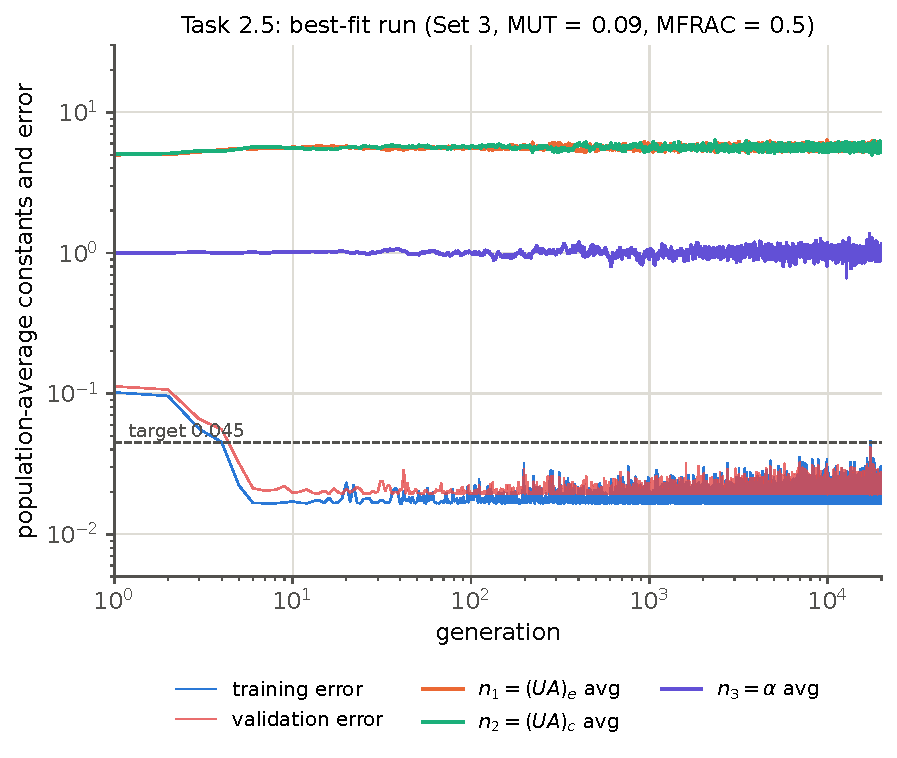
\includegraphics[width=0.7\linewidth]{figures/t25_evolution.pdf}
\caption{Task 2.5: evolution of the training and validation errors and of the population-average
constants for the best-fit run.}
\label{fig:t25evol}
\end{figure}

\begin{figure}[H]
\centering
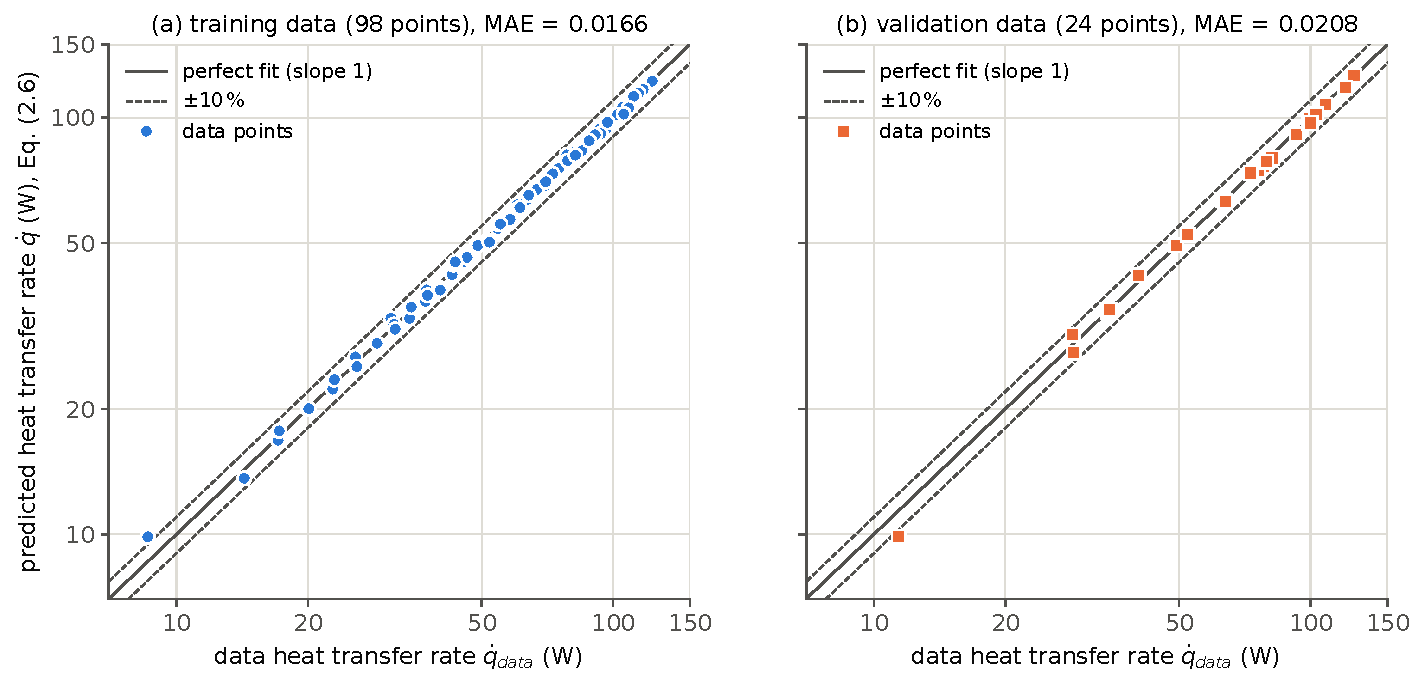
\includegraphics[width=\linewidth]{figures/t25_parity.pdf}
\caption{Task 2.5: predicted versus data heat transfer rate (log-log) for (a) the training data (circles)
and (b) the validation data (squares).}
\label{fig:t25parity}
\end{figure}

\begin{figure}[H]
\centering
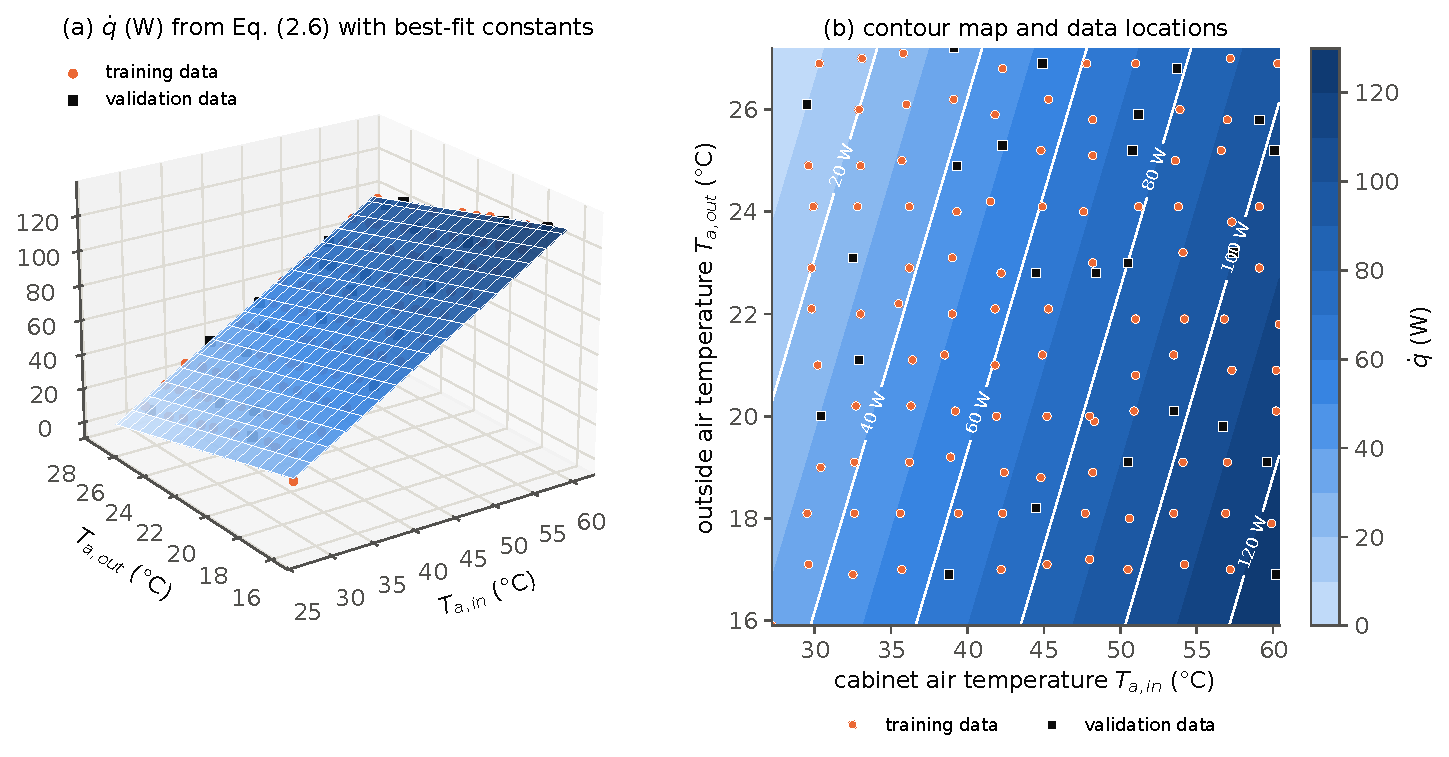
\includegraphics[width=\linewidth]{figures/t25_surface.pdf}
\caption{Task 2.5: heat transfer rate predicted by Eq.~(2.6) with the best-fit constants as a function of
$T_{a,in}$ and $T_{a,out}$ over the range of the data: (a) surface with the data points; (b) contour map.}
\label{fig:t25surf}
\end{figure}

\paragraph{How unique are $(UA)_e$, $(UA)_c$ and $\alpha$?}
Table~\ref{tab:t25study} shows that runs with the same error give quite different constants.
Figure~\ref{fig:t25deg} explains this. When $(UA)_e$ is fixed anywhere between 3.2 and 1000~W/\textdegree C and the
two other constants are re-optimised, the training MAE changes only from $\TwoFiveProfMinF$ to
$\TwoFiveProfMaxF$. The $\TwoFiveNconv$ converged GA runs give $(UA)_e=\TwoFiveConvNoneMin$--$\TwoFiveConvNoneMax$,
$(UA)_c=\TwoFiveConvNtwoMin$--$\TwoFiveConvNtwoMax$ and $\alpha=\TwoFiveConvNthreeMin$--$\TwoFiveConvNthreeMax$,
but the series conductance $UA_{eff}$ only varies between $\TwoFiveConvUAMin$ and $\TwoFiveConvUAMax$~W/\textdegree C
($\pm0.3\,\%$). The data contain only the overall conductance $UA_{eff}$ (two resistances in series)
and its weak temperature dependence through $h_r$. \textbf{They cannot separate the evaporator and
condenser conductances.} The final constants are therefore set by the initial guesses: the GA stops at the
point of the valley closest to where it started. Starting from equal guesses $(UA)_e=(UA)_c$, as for Set 3,
it returns nearly equal values ($5.7$ and $5.4$~W/\textdegree C). This is physically sensible, because the evaporator
and condenser fin sections of Fig.~2.1 have the same length (0.25~m). It also gives $\alpha\approx1.1$, so
radiation increases the condenser conductance by about $9\,\%$. To determine $(UA)_e$ and $(UA)_c$
separately, an additional measurement would be needed, e.g.\ the heat-pipe wall (vapour) temperature.

\begin{figure}[H]
\centering
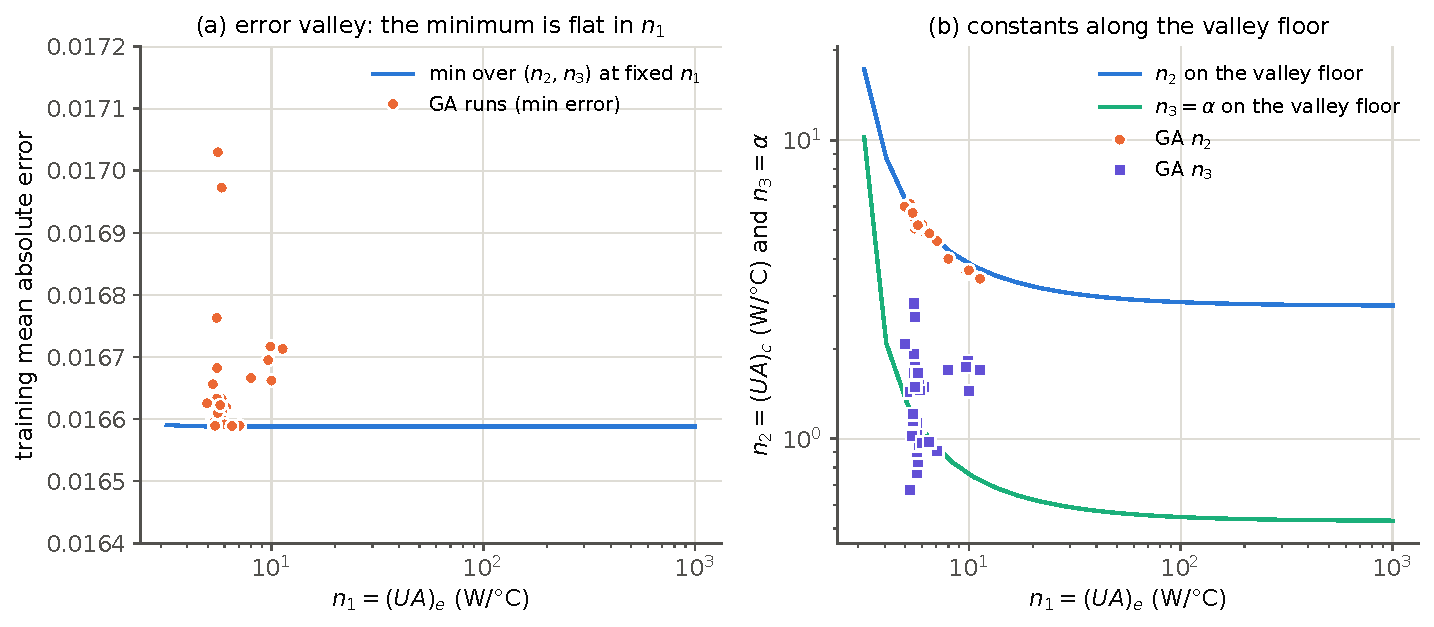
\includegraphics[width=\linewidth]{figures/t25_degeneracy.pdf}
\caption{Task 2.5: (a) minimum training error when $(UA)_e$ is fixed and $(UA)_c$, $\alpha$ are
re-optimised, with the converged GA runs; (b) values of $(UA)_c$ and $\alpha$ along the bottom of the
valley.}
\label{fig:t25deg}
\end{figure}

% ===============================================================
\section{Conclusions}
\label{sec:conclusions}
% ===============================================================

\subsection{Effect of the initial guesses on the stability and speed of convergence}
About 300 GA runs were made in this project (Tables~\ref{tab:t22study}, \ref{tab:t23study},
\ref{tab:t25study} and~\ref{tab:t25ngen}). Table~\ref{tab:concl} summarises how the initial guesses
of the constants affect the algorithm.

\begin{table}[H]
\centering\footnotesize
\caption{Summary: how the initial guesses affect the stability and the speed of convergence of the genetic
algorithm (MFRAC $=0.5$ and MUT $\approx\pm9\,\%$ unless stated).}
\label{tab:concl}
\begin{tabularx}{\linewidth}{@{}>{\raggedright\arraybackslash}p{3.3cm} >{\raggedright\arraybackslash}X >{\raggedright\arraybackslash}X >{\raggedright\arraybackslash}p{3.6cm}@{}}
\toprule
Initial guesses & Observed behaviour & Cause & Remedy\\
\midrule
Close to the solution (predicted output of the right order of magnitude): 2.2 Sets 1--2, 2.3 Set C, 2.5 Sets 3--4
& Stable. Target reached in \textbf{2--12 generations} in every run; final error within a few percent of the true minimum.
& Only the level of the prediction ($n_1$) has to be adjusted.
& Continue with small mutations to refine.\\
\addlinespace
Right order of magnitude but wrong position along a valley: 2.2 Set 1, 2.3 Set A
& Target reached quickly, but the constants depend on the guess and on the seed (e.g.\ $n_2=3.08$--$3.34$) and drift only slowly.
& Correlated constants ($\ln n_1$ and $n_2$; $n_3$, $n_4$ and $n_5$): long, flat valley of the error.
& Several seeds and guesses; larger MUT, then refinement; check the constants, not only the error.\\
\addlinespace
Far from the solution: 2.2 Sets 3--4, 2.3 Set D
& \textbf{Stagnation} at 2--4 times the minimum error. NGEN $=20000$ does not help. With MUT $=\pm40\,\%$: convergence after $\sim$130--1600 generations.
& Steps of at most $\pm$MUT per generation; most mutations away from the valley floor are rejected.
& Two stages: MUT $=0.2$--$0.4$ to explore, then MUT $=0.03$--$0.01$ to refine.\\
\addlinespace
All organisms with nearly the same large error: 2.3 Set E, 2.5 Sets 1--2 $(1,1,1)$, $(2,2,0.5)$
& \textbf{Population frozen}: nkeep $=0$ at every generation, error constant (0.6--0.95). Unaffected by MUT and NGEN.
& Relative threshold $0.5\times$median selects nobody; all offspring come from \code{n[0]}, which is never replaced.
& MFRAC $=1$ (converges in 55--84 generations), or better guesses.\\
\addlinespace
A constant guessed close to zero: 2.3 Set B ($n_5=0.01$)
& The constant stays near zero; only 3/10 runs reach the target.
& Multiplicative mutation: the step is proportional to the value.
& Guess a non-zero value of the expected order of magnitude.\\
\addlinespace
Constants not identifiable from the data: 2.5 ($(UA)_e$, $(UA)_c$, $\alpha$)
& Same error for $(UA)_e$ from 5 to 11~W/\textdegree C; the final constants follow the guess.
& The data only constrain the series conductance $UA_{eff}$.
& Report $UA_{eff}$; physically motivated guess $(UA)_e\approx(UA)_c$; more measurements.\\
\bottomrule
\end{tabularx}
\end{table}

In short:
\begin{enumerate}
  \item \textbf{The most important property of the initial guesses is that the model output they
        predict has the right order of magnitude.} When it does, the GA is stable and fast, whatever the
        exact values. When all organisms are far from the data, the relative selection threshold
        (MFRAC$\,\times\,$median) stops working and the skeleton algorithm can freeze completely.
  \item \textbf{Speed of convergence}: with good guesses, the target error is reached in a few to a few
        tens of generations, and the minimum is found within a few thousand generations. Beyond that,
        increasing NGEN does not help a trapped population. What helps is a larger mutation amplitude
        (exploration) followed by a small one (refinement), or a larger MFRAC.
  \item \textbf{Reaching the target error is not proof of an accurate fit.} With correlated constants,
        many sets of constants meet the target. To be confident, several seeds and initial guesses must give
        the same constants. The deterministic check showed that my best GA fits are within
        $0.03\,\%$ (Task~2.2), $0.6\,\%$ (Task~2.3) and $0.01\,\%$ (Task~2.5) of the true minimum error.
  \item \textbf{Constants that the data do not determine} (Task~2.5) stay at values that depend on the
        initial guess. Only identifiable combinations should be interpreted.
\end{enumerate}

\subsection{Main results}
\begin{itemize}
  \item \textbf{Task 2.2}: $\qpp=\TwoTwoNone\,\dTsat^{\TwoTwoNtwo}g^{\TwoTwoNthree}$, $\Ferrmean=\TwoTwoF$.
        The rms deviation ($\TwoTwoRmsRel\,\%$) is larger than the $\pm10\,\%$ uncertainty of the data, and
        the deviations are systematic between gravity levels. A power law in $g$ cannot represent the
        Marangoni effect.
  \item \textbf{Task 2.3}: $\qpp=\TwoThreeNone\,\dTsat^{\TwoThreeNtwo}(g+\TwoThreeNfour\,\gen\gamma)^{\TwoThreeNthree}P^{\TwoThreeNfive}$,
        $\Ferrmean=\TwoThreeF$ (validation $\TwoThreeFval$). The overall deviation is close to the noise
        level, but the $1\,\gen$ and $2\,\gen$ (5.5~kPa) groups keep a bias of $-16\,\%$ and $+11\,\%$. The
        Marangoni effect acts like an additional gravity of about $2.4\,\gen$ for $\gamma=1.79$, which
        explains why the heat flux hardly depends on gravity for this mixture.
  \item \textbf{ET1}: the heat flux is about 6 times more sensitive to the superheat than to pressure, the
        next most influential input. Keeping $|\Delta\qpp/\qpp|<0.15$ requires about $3.6\,\%$ accuracy on all inputs, or
        about $\pm1.4$--$1.9$\,\textdegree C on the superheat.
  \item \textbf{ET2}: the directly fitted inverse relation differs from the inverted forward relation by
        $\approx5$--$10\,\%$. This difference comes from the scatter of the data (regression dilution),
        as shown with synthetic data.
  \item \textbf{Tasks 2.4--2.5}: $(UA)_e=\TwoFiveNone$~W/\textdegree C, $(UA)_c=\TwoFiveNtwo$~W/\textdegree C, $\alpha=\TwoFiveNthree$.
        The MAE is $\TwoFiveFtrain$ for the training set and $\TwoFiveFval$ for the validation set, well
        below 0.045. Only the overall conductance $UA_{eff}=\TwoFiveUA$~W/\textdegree C is determined uniquely by the data.
\end{itemize}

% ===============================================================
\section{Summary of the program modifications (Task 2.6)}
\label{sec:codechanges}
% ===============================================================

This section lists, program by program, the modifications made to the previous version of the code, and
all the changes made to the basic structure of the example code. The complete programs are in
Appendix~\ref{app:code}. Every modified line is also marked in the code by a comment.

\subsection{Changes to the basic structure of the example code (all GA programs)}
\begin{enumerate}[label=\textbf{S\arabic*.}]
  \item \textbf{Bug fix -- \code{import random}.} In \code{CodeP2.2F26}, \code{import random} replaces the
        function \code{random()} imported in \code{CodeP2.1F26} by the module, so the combined program
        stops at the initialisation with a \code{TypeError}. It was replaced by
        \code{from random import random, seed}.
  \item \textbf{Data corrections.} Two values of \code{CodeP2.1F26} were corrected to match the Appendix
        (Table~\ref{tab:datacheck}).
  \item \textbf{Evolution loop placed in a function.} The skeleton code from ``INITIALIZING PARAMETERS'' to
        the final print was placed in \code{run\_GA(n1i,\dots,n5i, NGEN, MUT, MFRAC, rseed, target, verbose)}.
        This allows many runs (initial guesses, mutation amplitudes, seeds, NGEN) in the same notebook.
        Inside the function, the statements of the loop (fitness, selection, mating, mutation, averaging,
        minimum search, time averages) are those of the skeleton, line for line.
  \item \textbf{Parameters instead of literals.} The mutation amplitude (\code{0.085} in the code) is the
        argument \code{MUT}, and the selection fraction \code{MFRAC} ($=0.5$ in the skeleton) is an argument.
  \item \textbf{Reproducibility.} The skeleton seeds Python's \code{random} once but never seeds
        \code{numpy.random}, which is used for selection, mating and mutation. Every run therefore gave
        different results. \code{run\_GA} now calls \code{seed(rseed)} and \code{numpy.random.seed(rseed)},
        so any run of this report can be reproduced exactly from its seed.
  \item \textbf{Diagnostics returned.} The function returns the histories (\code{aFerrmeanavgn},
        \code{n1avg}, \dots), the generation of the minimum (\code{kmin}), the first generation below the
        target (\code{kconv}) and the number of survivors of each generation (\code{nkeephist}). None of
        these quantities affects the algorithm.
  \item \textbf{Figures.} The skeleton plots are kept (\code{plt.loglog()}, same legends). The
        \code{yticks} were extended down to $10^{-4}$ so that $n_1\approx10^{-3}$ is visible. Additional
        report-quality figures are saved as PDF files.
\end{enumerate}

\subsection{Program-by-program modifications}

\paragraph{\code{P2\_Task2.1} (from \code{CodeP2.1F26}).} S2; a print of the number of rows and of one
element; a cell that checks the data against the Appendix; a cell for the log-log plot and power-law
fits of Task~2.1(b).

\paragraph{\code{P2\_Task2.2} (from \code{CodeP2.1F26} + \code{CodeP2.2F26}).} S1--S7. The error
function of the skeleton (Eq.~(1.3)) is unchanged. Added cells: first run with the skeleton guesses,
deterministic reference, initial-guess study, best-fit plots and statistics, landscape.

\paragraph{\code{P2\_Task2.3} (copy of \code{P2\_Task2.2}).} Modifications (i)--(vii) of the statement:
\begin{enumerate}[label=(\roman*)]
  \item the red-text data lines (32 rows with $P=9.5$ and $7.0$~kPa, $\gamma=0$ and $1.71$) are
        uncommented, giving 77 rows;
  \item \code{ND = 77}, \code{NS = 77};
  \item the error function becomes Eq.~(1.7) in both locations (fitness loop and population-average loop),
        and the prediction used in the plots becomes Eq.~(1.5):
\begin{lstlisting}
gen_en = 9.8   # earth-normal gravitational acceleration, m/s2
Ferr[i] = n[i][0]*lydata[i][0] + math.log(n[i][1]) + n[i][2]*lydata[i][1]
Ferr[i] = Ferr[i] + n[i][3]*math.log( ydata[i][2] + n[i][4]*gen_en*ydata[i][3] ) + n[i][5]*lydata[i][4]
...
Ferravgn[i] = -1.*lydata[i][0] + math.log(n1avg[k]) + n2avg[k]*lydata[i][1]
Ferravgn[i] = Ferravgn[i] + n3avg[k]*math.log( ydata[i][2] + n4avg[k]*gen_en*ydata[i][3] ) + n5avg[k]*lydata[i][4]
...
qpred = n1*row[1]**n2 * (row[2] + n4*gen_en*row[3])**n3 * row[4]**n5
\end{lstlisting}
  \item the mating/mutation lines of $n_4$ and $n_5$ are uncommented (with amplitude \code{MUT});
  \item the final print-out lists $n_1$--$n_5$ (\code{ENDING}, \code{MINUMUM}, \code{TIME AVG});
  \item the legend of the first plot is replaced by the five-constant legend and $n_4$, $n_5$ are plotted;
  \item the default initial guesses are $0.000476,\ 3.028,\ 0.2249,\ 1.054,\ 0.217$.
\end{enumerate}
Added: the 15 validation points of the Appendix (\code{vdata}, used only to test the fit), the study
over initial guesses and the multi-stage refinement, the surface plot, and the profiles of
Fig.~\ref{fig:t23prof}.

\paragraph{\code{P2\_ET1} (new).} Reads the best-fit constants of Task~2.3 and evaluates the fractional
change ratios with finite steps, following steps 1--3 of the statement. It also computes the analytical
logarithmic derivatives and the limiting input inaccuracies.

\paragraph{\code{P2\_ET2} (copy of \code{P2\_Task2.3}).} The data rows are reorganised as
$[T_w-T_{sat},\ \qpp,\ g,\ \gamma,\ P]$ and \code{lydata} is recomputed. Because column~0 is now
$\ln\dTsat$ and column~1 is $\ln\qpp$, the error statements of Task~2.3 compute exactly the error of
Eq.~(ET2.1). Only the initial guesses (negative $\nh3$, $\nh5$: the multiplicative mutation keeps the
sign), the labels and the analysis cells were changed.

\paragraph{\code{P2\_Task2.4-2.5} (copy of \code{P2\_Task2.2}).}
\begin{itemize}
  \item The data are those of \code{CodeP2.3F26} (122 points $[T_{a,in},T_{a,out},\dot q]$). A seeded random
        permutation splits them into a training set (\code{ydata}, $N_D=98$, $80.3\,\%$) and a validation set
        (\code{vdata}, $N_V=24$, $19.7\,\%$). The GA sees only the training set, and $N_S=N_D=98$.
  \item The error function was changed in the two locations, Eqs.~(2.4)--(2.5), with $n_1=(UA)_e$,
        $n_2=(UA)_c$, $n_3=\alpha$. The model Eq.~(2.6) is coded once and used in both locations and in the plots:
\begin{lstlisting}
sigma = 5.67e-8     # Stefan-Boltzmann constant, W m-2 K-4
hcref = 80.0        # W m-2 K-1
def hrad(Tain, Taout):
    Ti = Tain + 273.15
    To = Taout + 273.15
    return sigma*(Ti + To)*(Ti**2 + To**2)
def qdot_model(n1, n2, n3, Tain, Taout):
    UAcr = n2*(1. + n3*hrad(Tain, Taout)/hcref)
    return UAcr*( n1*(Tain - Taout)/(n1 + UAcr) )
...
Ferr[i] = ydata[i][2] - qdot_model(n[i][1], n[i][2], n[i][3], ydata[i][0], ydata[i][1])
aFerr[i] = abs(Ferr[i])/abs(ydata[i][2])  #- absolute fractional error
...
Ferravgn[i] = ydata[i][2] - qdot_model(n1avg[k], n2avg[k], n3avg[k], ydata[i][0], ydata[i][1])
aFerravgn[i] = abs(Ferravgn[i])/abs(ydata[i][2])
\end{lstlisting}
  \item The mean absolute error of the validation set is computed at each generation with the
        population-average constants (\code{aFerrval}). It is used for monitoring only, not for selection.
  \item The plotting section was rewritten for the log-log plots of predicted versus data $\dot q$ (training
        and validation) and for the surface plot of $\dot q(T_{a,in},T_{a,out})$.
\end{itemize}


\appendix
% ===============================================================
\section{Programs}
\label{app:code}
% ===============================================================
This appendix lists all the programs (code cells of the Jupyter notebooks in \code{code/}, executed
in order). To avoid repeating the same code, a cell that is identical to a cell already listed (the data
cell \code{CodeP2.1F26} and the figure-style cell) is replaced by a reference to the first listing.
Modified or added lines are marked by comments. The executed notebooks, with all their outputs, are
provided with the report.

\subsection{Program A -- Task 2.1 (\code{P2\_Task2.1.ipynb})}
\lstinputlisting{code/P2_Task2_1.py}

\subsection{Program B -- Task 2.2 (\code{P2\_Task2.2.ipynb})}
\lstinputlisting{code/P2_Task2_2.py}

\subsection{Program C -- Task 2.3 (\code{P2\_Task2.3.ipynb})}
\lstinputlisting{code/P2_Task2_3.py}

\subsection{Program D -- Extra Task ET1 (\code{P2\_ET1.ipynb})}
\lstinputlisting{code/P2_ET1.py}

\subsection{Program E -- Extra Task ET2 (\code{P2\_ET2.ipynb})}
\lstinputlisting{code/P2_ET2.py}

\subsection{Program F -- Tasks 2.4 and 2.5 (\code{P2\_Task2.4-2.5.ipynb})}
\lstinputlisting{code/P2_Task2_4_2_5.py}


\end{document}
